\begin{chapterpage}{Introduction to linear regression}
  \chaptertitle{Introduction to linear \titlebreak{} regression}
  \label{linRegrForTwoVar}
  \label{ch_regr_simple_linear}
  \chaptersection{fitting_line_to_data_section}
  \chaptersection{fittingALineByLSR}
  \chaptersection{typesOfOutliersInLinearRegression}
  \chaptersection{inferenceForLinearRegression}
\end{chapterpage}
\renewcommand{\chapterfolder}{ch_regr_simple_linear}


\index{regression|textbf}
\index{regression|(}
\index{linear regression|seealso{regression}}

\chapterintro{Linear regression is a very powerful
  statistical technique.
  Many people have some familiarity with regression just from
  reading the news, where straight lines are overlaid
  on scatterplots.
  Linear models can be used for prediction or to
  evaluate whether there is a linear relationship
  between two numerical variables.}



%__________
\section{Fitting a line, residuals, and correlation}
% \section{Using a line to model data}
\label{fitting_line_to_data_section}

It's helpful to think deeply about the line fitting process.
In this section, we define the form of a linear model,
explore criteria for what makes a good fit,
and introduce a new statistic called
\emph{correlation}\index{correlation}.


\subsection{Fitting a line to data}

Figure~\ref{perfLinearModel} shows two variables whose
relationship can be modeled perfectly with a straight line.
The equation for the line is
\begin{eqnarray*}
y = 5 + 64.96 x
\end{eqnarray*}
Consider what a perfect linear relationship means:
we know the exact value of $y$ just by knowing
the value of $x$.
This is unrealistic in almost any natural process.
For example, if we took family income ($x$),
this value would provide some useful information about
how much financial support a college may offer a prospective
student~($y$).
However, the prediction would be far from perfect,
since other factors play a role in financial support
beyond a family's finances.

\begin{figure}[h]
   \centering
   \Figure{0.6}{perfLinearModel}
   \caption{Requests from twelve separate buyers were
       simultaneously placed with a trading company to purchase
       Target Corporation stock
       (ticker \texttt{TGT}, December 28th, 2018),
       and the total cost of the shares were reported.
       Because the cost is computed using a linear formula,
       the linear fit is perfect.}
   \label{perfLinearModel}
\end{figure}

Linear regression is the statistical method for fitting
a line to data where the relationship between two variables,
$x$ and $y$, can be modeled by a straight line with some error:
\begin{align*}
y = \beta_0 + \beta_1x + \varepsilon
\end{align*}
The values $\beta_0$ and $\beta_1$ represent the model's
parameters\index{parameter}
($\beta$ is the Greek letter
  \emph{beta}\index{Greek!beta@beta ($\beta$)}),
and the error is represented by $\varepsilon$
(the Greek letter \emph{epsilon}\index{Greek!epsilon@epsilon ($\varepsilon$)}).
The parameters are estimated using data,
and we write their point estimates as $b_0$ and $b_1$.
When we use $x$ to predict $y$,
we usually call $x$ the explanatory\index{explanatory variable}
or \term{predictor} variable,
and we call $y$ the response;
we also often drop the $\epsilon$ term when writing down the
model since our main focus is often on the prediction of
the average outcome.

It is rare for all of the data to fall perfectly on a straight line.
Instead, it's more common for data to appear as
a \emph{cloud of points}\index{cloud of points},
such as those examples shown in  Figure~\ref{imperfLinearModel}.
In each case, the data fall around a straight line,
even if none of the observations fall exactly on the line.
The first plot shows a relatively strong downward
linear trend,
where the remaining variability in the data around the
line is minor relative to the strength of the relationship
between $x$ and $y$.
The second plot shows an upward trend that,
while evident, is not as strong as the first.
The last plot shows a very weak downward trend in the data,
so slight we can hardly notice it.
In each of these examples,
we will have some uncertainty regarding our estimates
of the model parameters, $\beta_0$ and $\beta_1$.
For instance, we might wonder, should we move the line
up or down a little, or should we tilt it more or less?
As we move forward in this chapter,
we will learn about criteria for line-fitting,
and we will also learn about the uncertainty associated
with estimates of model parameters.

\begin{figure}
   \centering
   \Figure{}{imperfLinearModel}
   \caption{Three data sets where a linear model may be useful
       even though the data do not all fall exactly on the line.}
   \label{imperfLinearModel}
\end{figure}

There are also cases where fitting a straight line to the data,
even if there is a clear relationship between the variables,
is not helpful.
One such case is shown in
Figure~\ref{notGoodAtAllForALinearModel}
where there is a very clear relationship between the variables
even though the trend is not linear.
We discuss \index{nonlinear}nonlinear trends in this chapter
and the next, but details of fitting nonlinear models
are saved for a later course.

\begin{figure}
   \centering
   \Figure{0.8}{notGoodAtAllForALinearModel}
   \caption{A linear model is not useful in this nonlinear case.
       These data are from an introductory physics experiment.}
   \label{notGoodAtAllForALinearModel}
\end{figure}




\subsection{Using linear regression to predict possum head lengths}

\index{data!possum|(}

Brushtail possums are a marsupial that lives in Australia,
and a photo of one is shown in
Figure~\ref{brushtail_possum}.
Researchers captured 104 of these animals and took body
measurements before releasing the animals back into the wild.
We consider two of these measurements:
the total length of each possum, from head to tail,
and the length of each possum's head.

\setlength{\captionwidth}{0.83\mycaptionwidth}
\begin{figure}[h]
  \centering
  \Figure{0.5}{brushtail_possum}
  \caption{The common brushtail possum of Australia.\vspace{-1mm} \\
      -----------------------------\vspace{-2mm}\\
      {\footnotesize Photo by Greg Schechter
      (\oiRedirect{textbook-flickr_com_schechter_brushtail_possum_5653697137}
          {https://flic.kr/p/9BAFbR}).
      \oiRedirect{textbook-CC_BY_2}
          {CC~BY~2.0~license}.}}
  \label{brushtail_possum}
\end{figure}
\setlength{\captionwidth}{\mycaptionwidth}

%Scatterplots were introduced in Chapter~\ref{introductionToData}
%as a graphical technique to present two numerical variables
%simultaneously.
%Such plots permit the relationship between the variables
%to be examined with ease.
Figure~\ref{scattHeadLTotalL} shows a scatterplot for the head
length and total length of the possums.
Each point represents a single possum from the data.
The head and total length variables are associated:
possums with an above average total length also tend to have
above average head lengths.
While the relationship is not perfectly linear, it could
be helpful to partially explain the connection between these
variables with a straight line.

\D{\newpage}

\begin{figure}[h]
  \centering
  \Figure{0.75}{scattHeadLTotalL}
  \caption{A scatterplot showing head length against total length
      for 104 brushtail possums.
      A point representing a possum with head length 94.1mm
      and total length 89cm is highlighted.}
  \label{scattHeadLTotalL}
\end{figure}

%Straight lines should only be used when the data appear to have
%a linear relationship, such as the case shown in the left panel
%of Figure~\ref{scattHeadLTotalLTube}.
%The right panel of Figure~\ref{scattHeadLTotalLTube} shows
%a case where a curved line would be more useful in understanding
%the relationship between the two variables.

%\begin{figure}[h]
%  \centering
%  \Figure{0.95}{scattHeadLTotalLTube}
%  \caption{The figure on the left shows head length versus
%      total length, and reveals that many of the points could
%      be captured by a straight band.
%      On the right, we see that a curved band is more appropriate
%      in this scatterplot.}
%  \label{scattHeadLTotalLTube}
%\end{figure}

We want to describe the relationship between the head length and total length variables in the possum data set using a line. In this example, we will use the total length as the predictor variable, $x$, to predict a possum's head length, $y$. We could fit the linear relationship by eye, as in Figure~\ref{scattHeadLTotalLLine}. The equation for this line is
\begin{align*}
\hat{y} = 41 + 0.59x
\end{align*}
A ``hat'' on $y$ is used to signify that this is an estimate.
We can use this line to discuss properties of possums.
For instance, the equation predicts a possum with a total length
of 80 cm will have a head length of
\begin{align*}
\hat{y} &= 41 + 0.59\times 80 \\
	&= 88.2 % mm
\end{align*}
The estimate may be viewed as an average:
the equation predicts that possums with a total length of
80~cm will have an average head length of 88.2~mm.
Absent further information about an 80~cm possum,
the prediction for head length that uses the average
is a reasonable estimate.

\begin{figure}
  \centering
  \Figures{0.7}{scattHeadLTotalLLine}
      {scattHeadLTotalLLineResiduals}
  \caption{A reasonable linear model was fit to represent
      the relationship between head length and total length.}
  \label{scattHeadLTotalLLine}
\end{figure}

\begin{examplewrap}
\begin{nexample}{What other variables might help us predict the
    head length of a possum besides its length?}
  Perhaps the relationship would be a little different for
  male possums than female possums,
  or perhaps it would differ for possums from one region
  of Australia versus another region.
  In Chapter~\ref{ch_regr_mult_and_log},
  we'll learn about how we can include more than one predictor.
  Before we get there, we first need to better understand
  how to best build a simple linear model with one predictor.
\end{nexample}
\end{examplewrap}


\subsection{Residuals}

\index{residual|(}

\noindent%
\termsub{Residuals}{residual} are the leftover variation in the data after accounting for the model fit:
\begin{align*}
\text{Data} = \text{Fit} + \text{Residual}
\end{align*}
Each observation will have a residual, and three of the
residuals for the linear model we fit for the \data{possum}
data is shown in
Figure~\ref{scattHeadLTotalLLine}.
If an observation is above the regression line, then its residual,
the vertical distance from the observation to the line, is positive.
Observations below the line have negative residuals.
One goal in picking the right linear model is for these residuals
to be as small as possible.

%\begin{figure}[h]
%  \centering
%  \Figures{0.7}{scattHeadLTotalLLine}
%      {scattHeadLTotalLLineResiduals}
%  \caption{The linear model from
%      Figure~\ref{scattHeadLTotalLLine}
%      where 3 residuals are highlighted.}
%  \label{scattHeadLTotalLLineResiduals}
%\end{figure}

Let's look closer at the three residuals featured in
Figure~\ref{scattHeadLTotalLLine}.
The observation marked by an ``$\times$'' has a small,
negative residual of about -1;
the observation marked by ``$+$'' has a large residual of about +7;
and the observation marked by ``$\triangle$'' has a moderate
residual of about -4.
The size of a residual is usually discussed in terms of its
absolute value.
For example, the residual for ``$\triangle$'' is larger than
that of ``$\times$'' because $|-4|$ is larger than $|-1|$.

\begin{onebox}{Residual: difference between observed and expected}
The residual of the $i^{th}$ observation $(x_i, y_i)$ is the difference of the observed response ($y_i$) and the response we would predict based on the model fit ($\hat{y}_i$):
\begin{eqnarray*}
e_i = y_i - \hat{y}_i
\end{eqnarray*}
We typically identify $\hat{y}_i$ by plugging $x_i$ into the model.
\end{onebox}

\begin{examplewrap}
\begin{nexample}{The linear fit shown in Figure~\ref{scattHeadLTotalLLine} is given as $\hat{y} = 41 + 0.59x$. Based on this line, formally compute the residual of the observation $(77.0, 85.3)$. This observation is denoted by ``$\times$'' in Figure~\ref{scattHeadLTotalLLine}.
Check it against the earlier visual estimate,~-1.}
We first compute the predicted value of point ``$\times$'' based on the model:
\begin{eqnarray*}
\hat{y}_{\times} = 41+0.59x_{\times} = 41+0.59\times 77.0 = 86.4
\end{eqnarray*}
Next we compute the difference of the actual head length and the predicted head length:
\begin{eqnarray*}
e_{\times} = y_{\times} - \hat{y}_{\times} = 85.3 -  86.4 = -1.1
\end{eqnarray*}
The model's error is $e_{\times} = -1.1$mm,
which is very close to the visual estimate of -1mm.
The negative residual indicates that the linear model
overpredicted head length for this particular possum.
\end{nexample}
\end{examplewrap}

\begin{exercisewrap}
\begin{nexercise}
If a model underestimates an observation, will the residual be positive or negative? What about if it overestimates the observation?\footnotemark
\end{nexercise}
\end{exercisewrap}
\footnotetext{If a model underestimates an observation, then the model estimate is below the actual. The residual, which is the actual observation value minus the model estimate, must then be positive. The opposite is true when the model overestimates the observation: the residual is negative.}

\begin{exercisewrap}
\begin{nexercise}
Compute the residuals for the ``$+$'' observation $(85.0, 98.6)$
and the ``$\triangle$'' observation $(95.5, 94.0)$ in the figure
using the linear relationship $\hat{y} = 41 + 0.59x$.\footnotemark{}
\end{nexercise}
\end{exercisewrap}
\footnotetext{($+$) First compute the predicted value based on
  the model:
  \begin{align*}
  \hat{y}_{+} = 41+0.59x_{+} = 41+0.59\times 85.0 = 91.15
  \end{align*}
  Then the residual is given by
  \begin{align*}
  e_{+} = y_{+} - \hat{y}_{+} = 98.6-91.15=7.45
  \end{align*}
  This was close to the earlier estimate of 7.

\noindent%
($\triangle$) $\hat{y}_{\triangle} = 41+0.59x_{\triangle} = 97.3$.
$e_{\triangle} = y_{\triangle} - \hat{y}_{\triangle} = -3.3$,
close to the estimate of -4.}

Residuals are helpful in evaluating how well a linear model
fits a data set.
We often display them in a \term{residual plot} such as the
one shown in Figure~\ref{scattHeadLTotalLResidualPlot}
for the regression line in Figure~\ref{scattHeadLTotalLLine}.
The residuals are plotted at their original horizontal locations
but with the vertical coordinate as the residual.
For instance, the point $(85.0,98.6)_{+}$ had a residual
of 7.45, so in the residual plot it is placed at $(85.0, 7.45)$.
Creating a residual plot is sort of like tipping the
scatterplot over so the regression line is horizontal. 
\index{data!possum|)}

\begin{figure}[h]
  \centering
  \Figure{0.7}{scattHeadLTotalLResidualPlot}
  \caption{Residual plot for the model in
      Figure~\ref{scattHeadLTotalLLine}.}
  \label{scattHeadLTotalLResidualPlot}
\end{figure}

\D{\newpage}

\begin{examplewrap}
\begin{nexample}{One purpose of residual plots is to identify
    characteristics or patterns still apparent in data after
    fitting a model.
    Figure~\ref{sampleLinesAndResPlots} shows three scatterplots
    with linear models in the first row and residual plots in the
    second row.
    Can you identify any patterns remaining in the residuals?}

  In the first data set (first column), the residuals show
  no obvious patterns.
  The residuals appear to be scattered randomly around the
  dashed line that represents 0.

  The second data set shows a pattern in the residuals.
  There is some curvature in the scatterplot, which is more
  obvious in the residual plot.
  We should not use a straight line to model these data.
  Instead, a more advanced technique should be used.

  The last plot shows very little upwards trend, and the
  residuals also show no obvious patterns.
  It is reasonable to try to fit a linear model to the data.
  However, it is unclear whether there is statistically
  significant evidence that the slope parameter is different
  from zero.
  The point estimate of the slope parameter, labeled $b_1$,
  is not zero, but we might wonder if this could just be due
  to chance.
  We will address this sort of scenario in
  Section~\ref{inferenceForLinearRegression}.
\end{nexample}
\end{examplewrap}

\begin{figure}
   \centering
   \Figure{0.9}{sampleLinesAndResPlots}
   \caption{Sample data with their best fitting lines (top row) and their corresponding residual plots (bottom row).}
   \label{sampleLinesAndResPlots}
\end{figure}

\index{residual|)}


\subsection{Describing linear relationships with correlation}

\index{correlation|(}

\noindent%
We've seen plots with strong linear relationships and
others with very weak linear relationships.
It would be useful if we could quantify the strength of these
linear relationships with a statistic.

\begin{onebox}{Correlation: strength of a linear relationship}
  \termsub{Correlation}{correlation}, which always takes values
  between -1 and 1, describes the strength of the linear
  relationship between two variables.
  We denote the correlation by $R$.
\end{onebox}

We can compute the correlation using a formula, just as we did
with the sample mean and standard deviation.
This formula is rather complex,\footnote{Formally,
  we can compute the correlation for observations $(x_1, y_1)$,
  $(x_2, y_2)$, ..., $(x_n, y_n)$ using the formula
  \begin{align*}
  R = \frac{1}{n-1}
      \sum_{i=1}^{n} \frac{x_i-\bar{x}}{s_x}\frac{y_i-\bar{y}}{s_y}
  \end{align*}
  where $\bar{x}$, $\bar{y}$, $s_x$, and $s_y$ are the sample
  means and standard deviations for each variable.}
and like with other statistics, we generally perform the
calculations on a computer or calculator.
Figure~\ref{posNegCorPlots} shows eight plots and their
corresponding correlations.
Only when the relationship is perfectly linear is the
correlation either -1 or~1.
If~the relationship is strong and positive, the correlation
will be near~+1.
If~it is strong and negative, it will be near~-1.
If~there is no apparent linear relationship between the
variables, then the correlation will be near zero.

\begin{figure}
   \centering
   \Figure{0.9}{posNegCorPlots}
   \caption{Sample scatterplots and their correlations.
       The first row shows variables with a positive
       relationship, represented by the trend up and to
       the right.
       The second row shows variables with a negative trend,
       where a large value in one variable is associated with
       a low value in the other.}
   \label{posNegCorPlots}
\end{figure}

The correlation is intended to quantify the strength of a linear trend. Nonlinear trends, even when strong, sometimes produce correlations that do not reflect the strength of the relationship; see three such examples in Figure~\ref{corForNonLinearPlots}.

\begin{figure}[h]
   \centering
   \Figures{0.85}{posNegCorPlots}{corForNonLinearPlots}
   \caption{Sample scatterplots and their correlations.
       In each case, there is a strong relationship between
       the variables.
       However, because the relationship is nonlinear,
       the correlation is relatively weak.}
   \label{corForNonLinearPlots}
\end{figure}

\begin{exercisewrap}
\begin{nexercise}
No straight line is a good fit for the data sets
represented in Figure~\ref{corForNonLinearPlots}.
Try drawing nonlinear curves on each plot.
Once you create a curve for each, describe what is important
in your~fit.\footnotemark{}
\index{correlation|)}
\end{nexercise}
\end{exercisewrap}
\footnotetext{We'll leave it to you to draw the lines. In general, the lines you draw should be close to most points and reflect overall trends in the data.}

%\begin{examplewrap}
%\begin{nexample}{What other variables might help us predict the
%    head length of a possum besides its length?}
%  Perhaps the relationship would be a little different for
%  male possums than female possums,
%  as shown in Figure~\ref{scattHeadLTotalLSex},
%  Or perhaps it would differ for possums from one region
%  of Australia versus another region.
%  In Chapter~\ref{ch_regr_mult_and_log},
%  we'll learn about how we can include more than one predictor.
%  Before we get there, we first need to better understand
%  how to best build a simple linear model with one predictor.
%\end{nexample}
%\end{examplewrap}
%
%\begin{figure}
%  \centering
%  \Figure{0.6}{scattHeadLTotalLSex}
%  \caption{Possums where the possum's sex is represented
%      by the plotting icon.}
%  \label{scattHeadLTotalLSex}
%\end{figure}


{


%_______________
\newpage\subsection*{Exercises} % Line fitting, residuals, and correlation

% 1

\eoce{\qt{Visualize the residuals\label{visualize_residuals}} 
The scatterplots shown below each have a 
superimposed regression line. If we were to construct a residual plot 
(residuals versus $x$) for each, describe what those plots would look 
like.
\begin{center}
\includegraphics[width=0.42\textwidth]{ch_regr_simple_linear/figures/eoce/visualize_residuals/visualize_residuals_linear.pdf} 
\includegraphics[width=0.42\textwidth]{ch_regr_simple_linear/figures/eoce/visualize_residuals/visualize_residuals_fan_back.pdf}
\end{center}
}{}

% 2

\eoce{\qt{Trends in the residuals\label{trends_in_residuals}} 
Shown below are two plots of residuals 
remaining after fitting a linear model to two different sets of data. 
Describe important features and determine if a linear model would be 
appropriate for these data. Explain your reasoning.
\begin{center}
\includegraphics[width=0.42\textwidth]{ch_regr_simple_linear/figures/eoce/trends_in_residuals/trends_in_residuals_fan.pdf} 
\includegraphics[width=0.42\textwidth]{ch_regr_simple_linear/figures/eoce/trends_in_residuals/trends_in_residuals_log.pdf}
\end{center}
}{}

% 3

\eoce{\qt{Identify relationships, Part I\label{identify_relationships_1}} 
For each of the six plots, 
identify the strength of the relationship (e.g. weak, moderate, or 
strong) in the data and whether fitting a linear model would be 
reasonable.
\begin{center}
\includegraphics[width=0.32\textwidth]{ch_regr_simple_linear/figures/eoce/identify_relationships_1/identify_relationships_u.pdf}
\includegraphics[width=0.32\textwidth]{ch_regr_simple_linear/figures/eoce/identify_relationships_1/identify_relationships_lin_pos_strong.pdf}
\includegraphics[width=0.32\textwidth]{ch_regr_simple_linear/figures/eoce/identify_relationships_1/identify_relationships_lin_pos_weak.pdf}
\includegraphics[width=0.32\textwidth]{ch_regr_simple_linear/figures/eoce/identify_relationships_1/identify_relationships_n.pdf}
\includegraphics[width=0.32\textwidth]{ch_regr_simple_linear/figures/eoce/identify_relationships_1/identify_relationships_lin_neg_strong.pdf}
\includegraphics[width=0.32\textwidth]{ch_regr_simple_linear/figures/eoce/identify_relationships_1/identify_relationships_none.pdf}
\end{center}
}{}

% 4

\eoce{\qt{Identify relationships, Part II\label{identify_relationships_2}} 
For each of the six plots, 
identify the strength of the relationship (e.g. weak, moderate, or 
strong) in the data and whether fitting a linear model would be 
reasonable.
\begin{center}
\includegraphics[width=0.32\textwidth]{ch_regr_simple_linear/figures/eoce/identify_relationships_2/identify_relationships_s.pdf}
\includegraphics[width=0.32\textwidth]{ch_regr_simple_linear/figures/eoce/identify_relationships_2/identify_relationships_hockey_stick.pdf}
\includegraphics[width=0.32\textwidth]{ch_regr_simple_linear/figures/eoce/identify_relationships_2/identify_relationships_pos_lin_strong.pdf}
\includegraphics[width=0.32\textwidth]{ch_regr_simple_linear/figures/eoce/identify_relationships_2/identify_relationships_pos_weak.pdf}
\includegraphics[width=0.32\textwidth]{ch_regr_simple_linear/figures/eoce/identify_relationships_2/identify_relationships_pos_weaker.pdf}
\includegraphics[width=0.32\textwidth]{ch_regr_simple_linear/figures/eoce/identify_relationships_2/identify_relationships_neg_lin_weak.pdf}
\end{center}
}{}

% 5

\eoce{\qt{Exams and grades\label{exams_grades_correlation}} 
The two scatterplots below show the 
relationship between final and mid-semester exam grades recorded 
during several years for a Statistics course at a university.
\begin{parts}
\item Based on these graphs, which of the two exams has the strongest 
correlation with the final exam grade? Explain.
\item Can you think of a reason why the correlation between the exam 
you chose in part (a) and the final exam is higher?
\end{parts}
\begin{center}
\includegraphics[width=0.485\textwidth]{ch_regr_simple_linear/figures/eoce/exams_grades_correlation/exam_grades_1.pdf}
\hspace{0.02\textwidth}%
\includegraphics[width=0.485\textwidth]{ch_regr_simple_linear/figures/eoce/exams_grades_correlation/exam_grades_2.pdf}
\end{center}
}{}

% 6

\eoce{\qt{Husbands and wives, Part I\label{husbands_wives_correlation}}
The Great Britain Office of Population Census and Surveys once 
collected data on a random sample of 170 married couples in 
Britain, recording the age (in years) and heights (converted 
here to inches) of the husbands and wives.\footfullcite{Hand:1994} 
The scatterplot on the left shows the wife's age plotted against her 
husband's age, and the plot on the right shows wife's height 
plotted against husband's height.
\begin{center}
\includegraphics[width=0.38\textwidth]{ch_regr_simple_linear/figures/eoce/husbands_wives_correlation/husbands_wives_age.pdf} 
\hspace{5mm}
\includegraphics[width=0.38\textwidth]{ch_regr_simple_linear/figures/eoce/husbands_wives_correlation/husbands_wives_height.pdf}
\end{center}
\begin{parts}
\item Describe the relationship between husbands' and wives' ages.
\item Describe the relationship between husbands' and wives' heights.
\item Which plot shows a stronger correlation? Explain your reasoning.
\item Data on heights were originally collected in centimeters, and 
then converted to inches. Does this conversion affect the correlation 
between husbands' and wives' heights?
\end{parts}
}{}

% 7

\eoce{\noindent \begin{minipage}[c]{0.43\textwidth}
\qt{Match the correlation, Part I\label{match_corr_1}} 
\textbf{\color{red}FINAL FORMATTING REQUIRED.}
Match the calculated correlations to the corresponding scatterplot.
\begin{parts}
\item $r = -0.7$
\item $r = 0.45$ 
\item $r = 0.06$
\item $r = 0.92$
\end{parts} \vspace{21mm}
\end{minipage}
\begin{minipage}[c]{0.57\textwidth}
\begin{center}
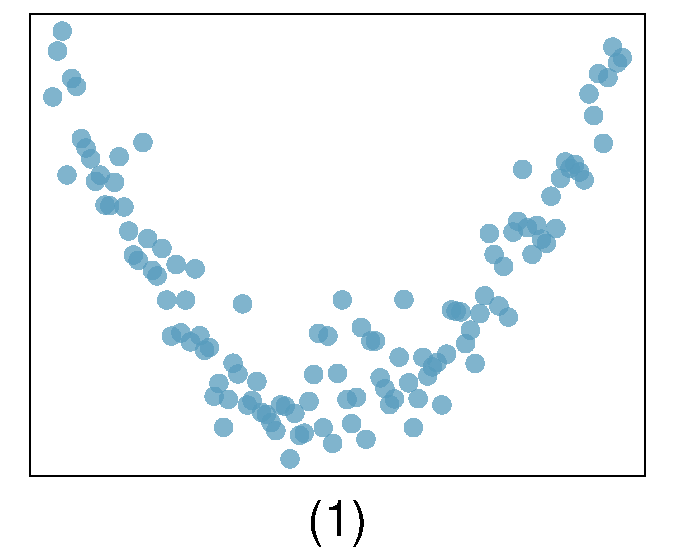
\includegraphics[width=0.45\textwidth]{ch_regr_simple_linear/figures/eoce/match_corr_1/match_corr_1_u.pdf}
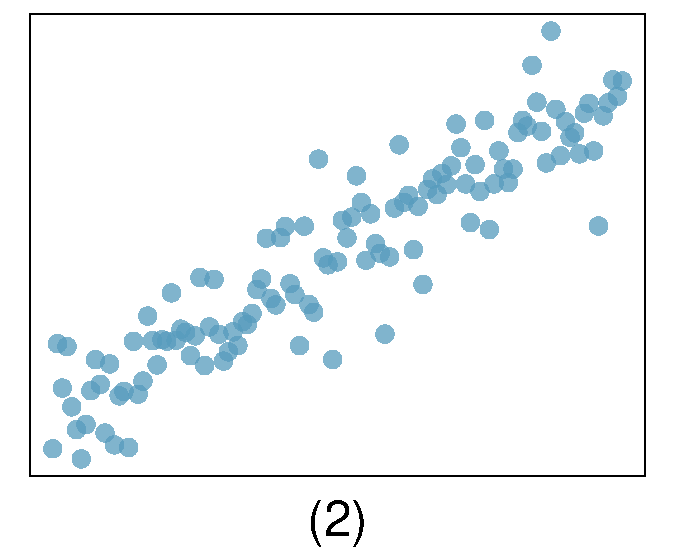
\includegraphics[width=0.45\textwidth]{ch_regr_simple_linear/figures/eoce/match_corr_1/match_corr_2_strong_pos.pdf} \\
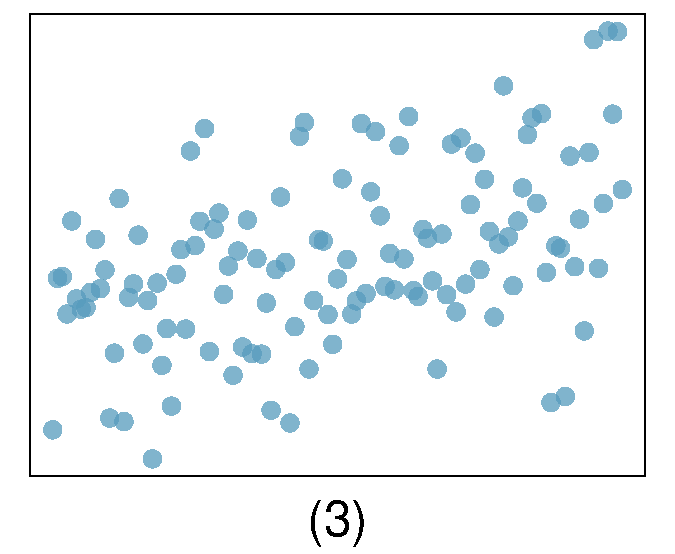
\includegraphics[width=0.45\textwidth]{ch_regr_simple_linear/figures/eoce/match_corr_1/match_corr_3_weak_pos.pdf}
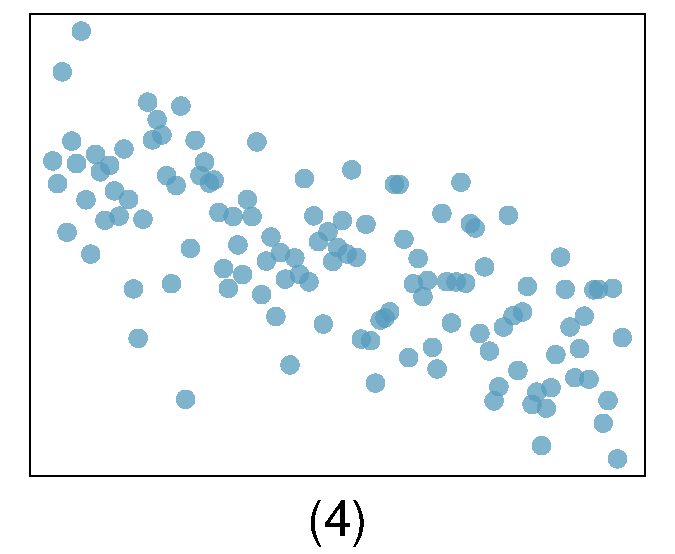
\includegraphics[width=0.45\textwidth]{ch_regr_simple_linear/figures/eoce/match_corr_1/match_corr_4_weak_neg.pdf}
\end{center}
\end{minipage}
}{}

% 8

\eoce{\noindent \begin{minipage}[c]{0.43\textwidth}
\qt{Match the correlation, Part II\label{match_corr_2}} 
\textbf{\color{red}FINAL FORMATTING REQUIRED.}
Match the calculated correlations to the corresponding scatterplot.
\begin{parts}
\item $r = 0.49$
\item $r = -0.48$ 
\item $r = -0.03$ 
\item $r = -0.85$
\end{parts} \vspace{21mm}
\end{minipage}
\begin{minipage}[c]{0.57\textwidth}
\begin{center}
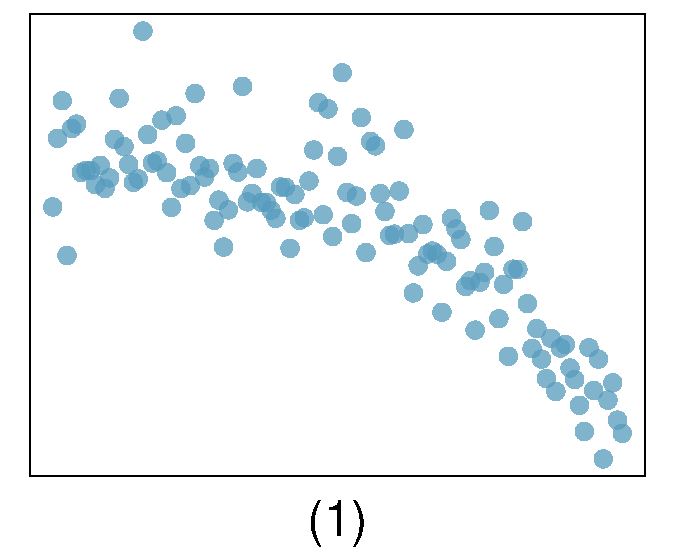
\includegraphics[width=0.45\textwidth]{ch_regr_simple_linear/figures/eoce/match_corr_2/match_corr_1_strong_neg_curved.pdf}
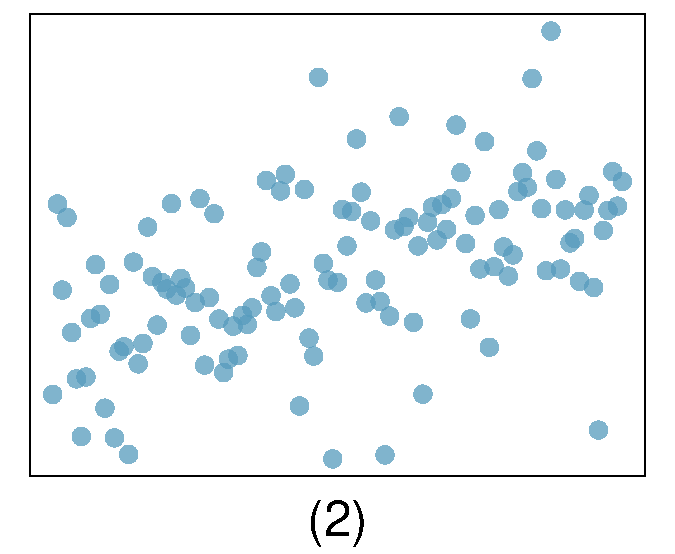
\includegraphics[width= 0.45\textwidth]{ch_regr_simple_linear/figures/eoce/match_corr_2/match_corr_2_weak_pos.pdf} \\
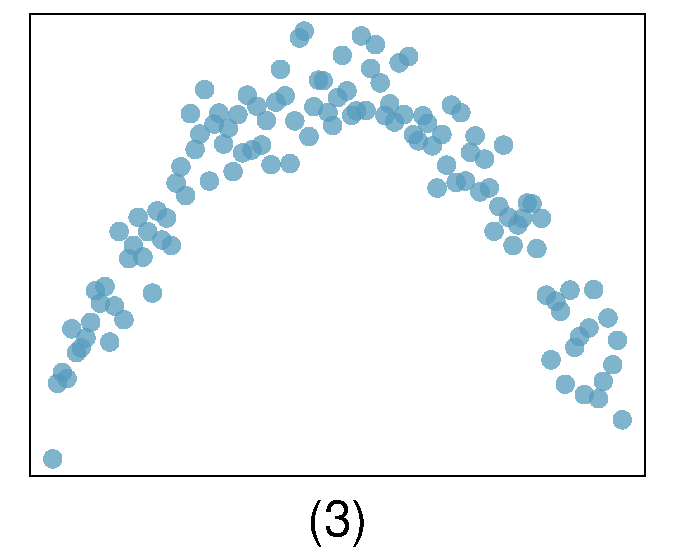
\includegraphics[width= 0.45\textwidth]{ch_regr_simple_linear/figures/eoce/match_corr_2/match_corr_3_n.pdf}
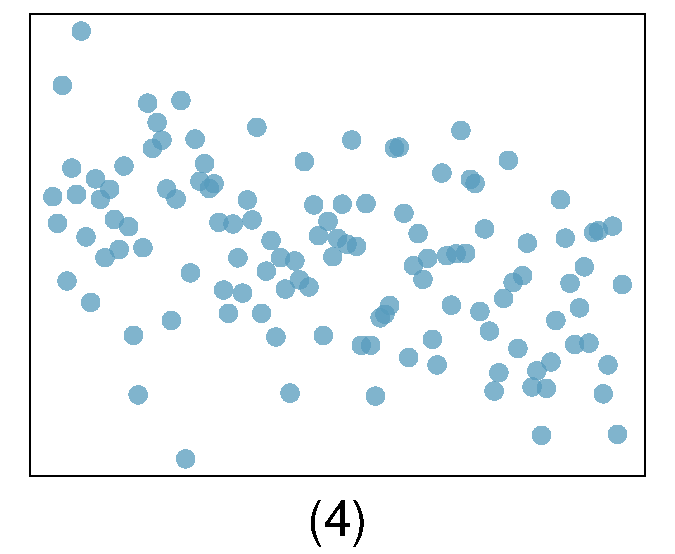
\includegraphics[width= 0.45\textwidth]{ch_regr_simple_linear/figures/eoce/match_corr_2/match_corr_4_weak_neg.pdf}
\end{center}
\end{minipage}
}{}

% 9

\eoce{\qt{Guess the correlation\label{guess_correlation}} Eduardo and Rosie 
are both collecting data on number of rainy days in a year and the total 
rainfall for the year. Eduardo records rainfall in inches and Rosie in 
centimeters. How will their correlation coefficients compare?
}{}

% 10

\eoce{\qt{Speed and height\label{speed_height_gender}} 1,302 UCLA students 
were asked to fill out a survey where they were asked about their height, 
fastest speed they have ever driven, and gender. The scatterplot on the 
left displays the relationship between height and fastest speed, and 
the scatterplot on the right displays the breakdown by gender in 
this relationship.
\begin{center}
\includegraphics[width=0.485\textwidth]{ch_regr_simple_linear/figures/eoce/speed_height_gender/speed_height.pdf}
\hspace{0.02\textwidth}%
\includegraphics[width=0.485\textwidth]{ch_regr_simple_linear/figures/eoce/speed_height_gender/speed_height_gender.pdf}
\end{center}
\begin{parts}
\item Describe the relationship between height and fastest speed.
\item Why do you think these variables are positively associated?
\item What role does gender play in the relationship between height 
and fastest driving speed?
\end{parts}
}{}

% 11

\eoce{\qt{The Coast Starlight, Part I\label{coast_starlight_corr_units}} 
The Coast Starlight Amtrak train runs from Seattle to Los Angeles. 
The scatterplot below displays the distance between each stop 
(in miles) and the amount of time it takes to travel from one stop 
to another (in minutes).\vspace{2mm}

\noindent\begin{minipage}[c]{0.485\textwidth}
\begin{parts}
\item Describe the relationship between distance and travel time.
\item How would the relationship change if travel time was instead measured 
in hours, and distance was instead measured in kilometers?
\item Correlation between travel time (in miles) and distance (in minutes) 
is $r = 0.636$. What is the correlation between travel time (in kilometers) 
and distance (in hours)?
\end{parts} \vspace{7mm}
\end{minipage}
\begin{minipage}[c]{0.02\textwidth}
$\:$\\
\end{minipage}
\begin{minipage}[c]{0.485\textwidth}
\includegraphics[width=\textwidth]{ch_regr_simple_linear/figures/eoce/coast_starlight_corr_units/coast_starlight.pdf}
\end{minipage}
}{}

% 12

\eoce{\qt{Crawling babies, Part I\label{crawling_babies_corr_units}}  
A study conducted at the University of Denver investigated whether babies 
take longer to learn to crawl in cold months, when they are often bundled 
in clothes that restrict their movement, than in warmer months.
\footfullcite{Benson:1993} Infants born during the study year were split 
into twelve groups, one for each birth month. We consider the average 
crawling age of babies in each group against the average temperature when 
the babies are six months old (that's when babies often begin trying to 
crawl). Temperature is measured in degrees Fahrenheit (\degree F) and age 
is measured in weeks.\vspace{2mm}

\noindent\begin{minipage}[c]{0.485\textwidth}
\begin{parts}
\item Describe the relationship between temperature and crawling age.
\item How would the relationship change if temperature was measured in 
degrees Celsius (\degree C) and age was measured in months?
\item The correlation between temperature in \degree F and age in weeks 
was $r=-0.70$. If we converted the temperature to \degree C and age to 
months, what would the correlation be?
\end{parts} \vspace{3mm}
\end{minipage}
\begin{minipage}[c]{0.02\textwidth}
$\:$\\
\end{minipage}
\begin{minipage}[c]{0.485\textwidth}
\includegraphics[width=\textwidth]{ch_regr_simple_linear/figures/eoce/crawling_babies_corr_units/crawling_babies.pdf}
\end{minipage}
}{}

% 13

\eoce{\qt{Body measurements, Part I\label{body_measurements_shoulder_height_corr_units}} 
Researchers studying anthropometry collected body girth measurements and 
skeletal diameter measurements, as well as age, weight, height and gender 
for 507 physically active individuals.\footfullcite{Heinz:2003} The 
scatterplot below shows the relationship between height and shoulder 
girth (over deltoid muscles), both measured in centimeters. \\[3mm]

\begin{minipage}[c]{0.485\textwidth}
\begin{parts}
\item Describe the relationship between shoulder girth and height.
\item How would the relationship change if shoulder girth was measured 
in inches while the units of height remained in centimeters?
\end{parts}\vspace{20mm}
\end{minipage}
\begin{minipage}[c]{0.02\textwidth}                  
$\:$\\
\end{minipage}
\begin{minipage}[c]{0.485\textwidth}
\includegraphics[width=\textwidth]{ch_regr_simple_linear/figures/eoce/body_measurements_shoulder_height_corr_units/body_measurements_height_shoulder_girth.pdf}
\end{minipage}
}{}

% 14

\eoce{\qt{Body measurements, Part II\label{body_measurements_hip_weight_corr_units}} 
The scatterplot below shows the relationship between weight 
measured in kilograms and hip girth measured in centimeters 
from the data described in 
Exercise~\ref{body_measurements_shoulder_height_corr_units}. \\[1mm]

\begin{minipage}[c]{0.485\textwidth}
\begin{parts}
\item Describe the relationship between hip girth and weight.
\item How would the relationship change if weight was measured in pounds 
while the units for hip girth remained in centimeters?
\end{parts}\vspace{20mm}
\end{minipage}
\begin{minipage}[c]{0.02\textwidth}
$\:$\\
\end{minipage}
\begin{minipage}[c]{0.485\textwidth}
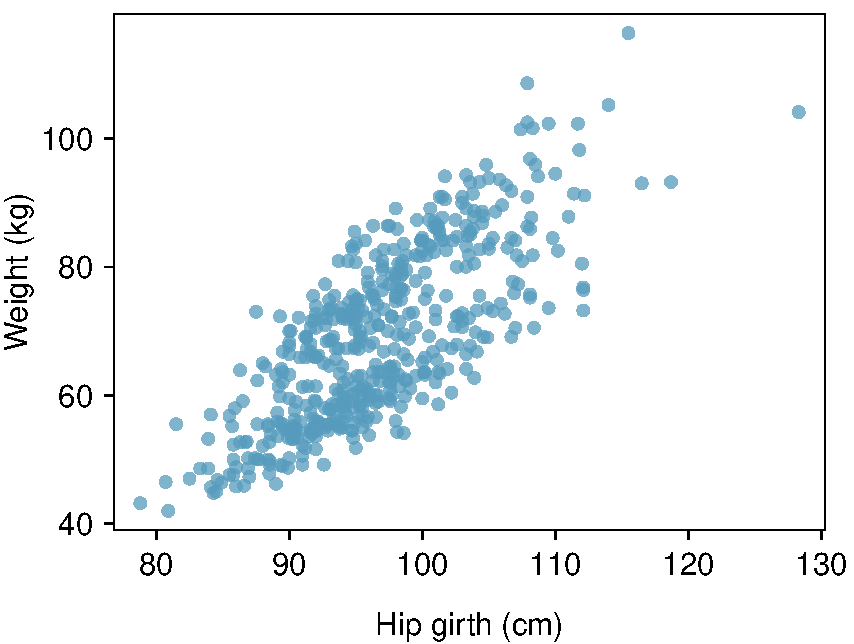
\includegraphics[width=\textwidth]{ch_regr_simple_linear/figures/eoce/body_measurements_hip_weight_corr_units/body_measurements_weight_hip_girth.pdf}
\end{minipage}
}{}

% 15

\eoce{\qt{Correlation, Part I\label{corr_husband_wife_age}} What would be the 
correlation between the ages of husbands and wives if men always married 
woman who were
\begin{parts}
\item 3 years younger than themselves? 
\item 2 years older than themselves? 
\item half as old as themselves?
\end{parts}
}{}

% 16

\eoce{\qt{Correlation, Part II\label{corr_men_women_salary}} What would be the 
correlation between the annual salaries of males and females at a company 
if for a certain type of position men always made
\begin{parts}
\item \$5,000 more than women?
\item 25\% more than women?
\item 15\% less than women?
\end{parts}
}{}
}







%__________________
\section{Least squares regression}
\label{fittingALineByLSR}

\index{least squares regression|(}

Fitting linear models by eye is open to criticism since
it is based on an individual's preference.
In this section, we use \emph{least squares regression}
as a more rigorous approach.


\subsection{Gift aid for freshman at Elmhurst College}

This section considers family income and gift aid data from
a random sample of fifty students in the freshman class of
Elmhurst College in Illinois.
Gift aid is financial aid that does not need to be paid back,
as opposed to a loan.
A scatterplot of the data is shown in
Figure~\ref{elmhurstScatterW2Lines}
along with two linear fits.
The lines follow a negative trend in the data;
students who have higher family incomes tended to have lower
gift aid from the university.

\begin{figure}[h]
  \centering
  \Figures{0.67}{elmhurstPlots}{elmhurstScatterW2Lines}
  \caption{Gift aid and family income for a random sample of
      50~freshman students from Elmhurst College.
      Two lines are fit to the data, the solid line being the
      \emph{least squares line}.}
  \label{elmhurstScatterW2Lines}
\end{figure}

\begin{exercisewrap}
\begin{nexercise}
Is the correlation positive or negative in Figure~\ref{elmhurstScatterW2Lines}?\footnotemark
\end{nexercise}
\end{exercisewrap}
\footnotetext{Larger family incomes are associated with lower amounts of aid, so the correlation will be negative. Using a computer, the correlation can be computed: -0.499.}


\subsection{An objective measure for finding the best line}

We begin by thinking about what we mean by ``best''.
Mathematically, we want a line that has small residuals.
The first option that may come to mind is to minimize the
sum of the residual magnitudes:
\begin{align*}
|e_1| + |e_2| + \dots + |e_n|
\end{align*}
which we could accomplish with a computer program.
The resulting dashed line shown in
Figure~\ref{elmhurstScatterW2Lines}
demonstrates this fit can be quite reasonable.
However, a more common practice is to choose the line that
minimizes the sum of the squared residuals:
\begin{align*}
e_{1}^2 + e_{2}^2 + \dots + e_{n}^2
\end{align*}


The line that minimizes this \term{least squares criterion}
is represented as the solid line in
Figure~\ref{elmhurstScatterW2Lines}.
This is commonly called the \term{least squares line}.
The following are three possible reasons to choose this option
instead of trying to minimize the sum of residual magnitudes
without any squaring:
\begin{enumerate}
\item
    It is the most commonly used method.
\item
    Computing the least squares line is widely supported
    in statistical software.
\item
    In many applications, a residual twice as large
    as another residual is more than twice as bad.
    For example, being off by 4 is usually more than twice
    as bad as being off by 2.
    Squaring the residuals accounts for this discrepancy.
\end{enumerate}
The first two reasons are largely for tradition and convenience;
the last reason explains why the least squares criterion
is typically most helpful.\footnote{There
  are applications where the sum of residual magnitudes
  may be more useful, and there are plenty of other criteria
  we might consider.
  However, this book only applies the least squares criterion.}


\subsection{Conditions for the least squares line}

\noindent%
When fitting a least squares line, we generally require
\begin{description}
\setlength{\itemsep}{0mm}
\item[Linearity.]
    The data should show a linear trend.
    If there is a nonlinear trend (e.g. left panel of
    Figure~\ref{whatCanGoWrongWithLinearModel}),
    an advanced regression method from another book
    or later course should be applied.
\item[Nearly normal residuals.]
    Generally, the residuals must be nearly normal.
    When this condition is found to be unreasonable,
    it is usually because of outliers or concerns
    about influential points,
%    The theoretical condition is that the residuals
%    must be normally distributed.
%    The importance of this condition depends on a few factors:
%    \begin{enumerate}[(1)]
%    \item
%        Is there any interest in predicting the range of
%        plausible values for individual observations?
%        If yes, then normality is important.
%    \item
%        Are there very few observations, such as fewer than~30?
%        If yes, then normality is important.
%    \end{enumerate}
%    If the answer is \emph{no} to each of these questions,
%    then
%    However, this condition can be taken with a grain of salt
%    when primarily focused on the trend of the data.
%    When the data's trend is the focus,
%    the number of observations can be modest in number,
%    such as 30 or more, at which point this condition
%    can be somewhat relaxed.
%    Generally, it is important to look for outliers,
    which we'll talk about more in
    Sections~\ref{typesOfOutliersInLinearRegression}.
    An example of a residual that would be a potentially
    concern is shown in
    Figure~\ref{whatCanGoWrongWithLinearModel},
    where one observation is clearly much further from the
    regression line than the others.
\item[Constant variability.]
    The variability of points around the least squares line
    remains roughly constant.
    An example of non-constant variability is shown in the
    third panel of Figure~\ref{whatCanGoWrongWithLinearModel},
    which represents the most common pattern observed
    when this condition fails:
    the variability of $y$ is larger when $x$ is larger.
\item[Independent observations.]
    Be cautious about applying regression to \term{time series}
    data, which are sequential observations in time such as a
    stock price each day.
    Such data may have an underlying structure that should
    be considered in a model and analysis.
    An example of a data set where successive observations
    are not independent is shown in the fourth panel of
    Figure~\ref{whatCanGoWrongWithLinearModel}.
    There are also other instances where correlations within
    the data are important, which is further discussed in
    Chapter~\ref{ch_regr_mult_and_log}.
\end{description}

\begin{figure}[h]
  \centering
  \Figure{}{whatCanGoWrongWithLinearModel}
  \caption{Four examples showing when the methods in this
      chapter are insufficient to apply to the data.
      First panel: linearity fails.
      Second panel: there are outliers, most especially
      one point that is very far away from the line.
      Third panel: the variability of the errors is related
      to the value of $x$.
      Fourth panel: a time series data set is shown,
      where successive observations are highly correlated.}
  \label{whatCanGoWrongWithLinearModel}
\end{figure}

\begin{exercisewrap}
\begin{nexercise}
Should we have concerns about applying least squares regression to the Elmhurst data in Figure~\ref{elmhurstScatterW2Lines}?\footnotemark
\end{nexercise}
\end{exercisewrap}
\footnotetext{The trend appears to be linear, the data fall around the line with no obvious outliers, the variance is roughly constant. These are also not time series observations. Least squares regression can be applied to these data.}


\D{\newpage}

\subsection{Finding the least squares line}
\label{findingTheLeastSquaresLineSection}

For the Elmhurst data, we could write the equation of the least squares regression line as
\begin{eqnarray*}
\widehat{aid} = \beta_0 + \beta_{1}\times
    \textit{family\us{}income}
\end{eqnarray*}
Here the equation is set up to predict gift aid based on a student's family income, which would be useful to students considering Elmhurst. These two values, $\beta_0$ and $\beta_1$, are the parameters\index{parameter} of the regression line.

As in
Chapters~\ref{ch_foundations_for_inf},
\ref{ch_inference_for_props},
and~\ref{ch_inference_for_means},
the parameters are estimated using observed data. In practice, this estimation is done using a computer in the same way that other estimates, like a sample mean, can be estimated using a computer or calculator. However, we can also find the parameter estimates by applying two properties of the least squares line:
\begin{itemize}
\item
    The slope of the least squares line can be estimated by
    \begin{align*}
    b_1 = \frac{s_y}{s_x} R
    \end{align*}
    where $R$ is the correlation between the two variables,
    and $s_x$ and $s_y$ are the sample standard deviations
    of the explanatory variable and response, respectively.
\item
    If $\bar{x}$ is the sample mean of the explanatory variable
    and $\bar{y}$ is the sample mean of the vertical variable,
    then the point $(\bar{x}, \bar{y})$ is on the least squares
    line.

    Figure~\ref{summaryStatsElmhurstRegr} shows the sample means
    for the family income and gift aid as \$101,780 and \$19,940,
    respectively.
    We could plot the point $(101.8, 19.94)$ on
    Figure~\vref{elmhurstScatterW2Lines}
    to verify it falls on the least squares line (the solid line).
%     and from the point-slope formula, we can identify $b_0$:
%    \begin{align*}
%    \hat{y} - \bar{y} = b_1 (x - \bar{x})
%    \qquad \to \qquad
%    \hat{y} = (\bar{y} - b_1 \bar{x}) + b_1 x
%    \end{align*}
%    This is the point-slope form of a line,
%    where $b_0 = \bar{y} - b_1 \bar{x}$.
\end{itemize}
Next, we formally find the point estimates $b_0$ and $b_1$
of the parameters $\beta_0$ and $\beta_1$.


\begin{figure}[ht]
\centering
\begin{tabular}{l rr}
\hline
\vspace{-4mm} & & \\
\vspace{0.4mm}	&	\ \ Family Income ($x$)	&
    \ \ Gift Aid ($y$) \\
\hline
  \vspace{-3.9mm} & & \\
mean & $\bar{x} = \text{\$101,780}$ &
    $\bar{y} = \text{\$19,940}$ \\
sd & $s_x = \text{\$63,200}$ &
    $s_y = \text{\$5,460}$ \vspace{0.4mm} \\
\hline
\vspace{-4mm}\ &\\
	& \multicolumn{2}{r}{$R=-0.499$} \\
\hline
\end{tabular}
\caption{Summary statistics for family income and gift aid.}
\label{summaryStatsElmhurstRegr}
\end{figure}

\D{\newpage}

\begin{exercisewrap}
\begin{nexercise} \label{findingTheSlopeOfTheLSRLineForIncomeAndAid}
Using the summary statistics in Figure~\ref{summaryStatsElmhurstRegr}, compute the slope for the regression line of gift aid against family income.\footnotemark
\end{nexercise}
\end{exercisewrap}
\footnotetext{Compute the slope using the summary statistics from Figure~\ref{summaryStatsElmhurstRegr}:
\begin{eqnarray*}
b_1
  = \frac{s_y}{s_x} R
  = \frac{\text{5,460}}{\text{63,200}}(-0.499)
  = -0.0431
\end{eqnarray*}}

You might recall the \term{point-slope} form of a line
from math class, which we can use to find the model fit,
including the estimate of $b_0$.
Given the slope of a line and a point on the line,
$(x_0, y_0)$, the equation for the line can be written as
\begin{align*}
y - y_0 = slope\times (x - x_0)
\end{align*}
%We could plug in $(\bar{x}, \bar{y})$ in for $(x_0, y_0$ and solve for $\hat{y}$ to arrive at the model.
%A common exercise to become more familiar with foundations of least squares regression is to use basic summary statistics and point-slope form to produce the least squares line. 

\begin{onebox}{Identifying the least squares line from summary statistics}
To identify the least squares line from summary statistics:\vspace{-1mm}
\begin{itemize}
\setlength{\itemsep}{0mm}
\item
    Estimate the slope parameter, $b_1 = (s_y / s_x) R$.
\item
    Noting that the point $(\bar{x}, \bar{y})$ is on the least
    squares line, use $x_0 = \bar{x}$ and $y_0 = \bar{y}$ with
    the point-slope equation: $y - \bar{y} = b_1 (x - \bar{x})$.
\item
    Simplify the equation, which would reveal that
    $b_0 = \bar{y} - b_1 \bar{x}$.
\end{itemize}
\end{onebox}

\begin{examplewrap}
\begin{nexample}{Using the point $(101780, 19940)$
    from the sample means and the slope estimate
    $b_1 = -0.0431$ from Guided
    Practice~\ref{findingTheSlopeOfTheLSRLineForIncomeAndAid},
    find the least-squares line for predicting aid based
    on family income.}
  \label{exampleToFindLSRLineOfElmhurstData}%
  Apply the point-slope equation using $(101.8, 19.94)$
  and the slope $b_1 = -0.0431$:
  \begin{align*}
  y - y_0    &= b_1 (x - x_0) \\
  y - \text{19,940}  &= -0.0431(x - \text{101,780})
  \end{align*}
  Expanding the right side and then adding 19,940 to each side,
  the equation simplifies:
  \begin{align*}
  \widehat{aid} = \text{24,320} - 0.0431 \times
      \textit{family\us{}income}
  \end{align*}
  Here we have replaced $y$ with $\widehat{aid}$ and $x$ with
  \textit{family\us{}income} to put the equation in context.
  The final equation should always include a ``hat''
  on the variable being predicted, whether it is a generic
  ``$y$'' or a named variable like ``$aid$''.
\end{nexample}
\end{examplewrap}

A computer is usually used to compute the least squares line,
and a summary table generated using software for the Elmhurst
regression line is shown in
Figure~\ref{rOutputForIncomeAidLSRLine}.
The first column of numbers provides estimates for ${b}_0$
and ${b}_1$, respectively.
These results match those from
Example~\ref{exampleToFindLSRLineOfElmhurstData}.

\begin{figure}[ht]
\centering
\begin{tabular}{l rrrr}
  \hline
  \vspace{-3.7mm} & & & & \\
 & Estimate & Std. Error & t value & Pr($>$$|$t$|$) \\ 
  \hline
  \vspace{-3.6mm} & & & & \\
(Intercept) & 24319.3 & 1291.5 & 18.83 & $<$0.0001 \\ 
family\us{}income & -0.0431 & 0.0108 & -3.98 & 0.0002 \\ 
  \hline
\end{tabular}
\caption{Summary of least squares fit for the Elmhurst data.
    Compare the parameter estimates in the first column to
    the results of
    Example~\ref{exampleToFindLSRLineOfElmhurstData}.}
\label{rOutputForIncomeAidLSRLine}
\end{figure}

\D{\newpage}

\begin{examplewrap}
\begin{nexample}{Examine the second, third, and fourth columns
    in Figure~\ref{rOutputForIncomeAidLSRLine}.
    Can you guess what they represent?
    (If you have not reviewed any inference chapter yet,
    skip this example.)}
  We'll describe the meaning of the columns using the
  second row, which corresponds to~$\beta_1$.
  The first column provides the point estimate for $\beta_1$,
  as we calculated in an earlier example: $b_1 = -0.0431$.
  The second column is a standard error for this point estimate:
  $SE_{b_1} = 0.0108$.
  The third column is a $t$-test statistic for the null
  hypothesis that $\beta_1 = 0$: $T = -3.98$.
  The last column is the p-value for the $t$-test statistic
  for the null hypothesis $\beta_1 = 0$ and a two-sided
  alternative hypothesis: 0.0002.
  We will get into more of these details in
  Section~\ref{inferenceForLinearRegression}.
\end{nexample}
\end{examplewrap}

\begin{examplewrap}
\begin{nexample}{Suppose a high school senior is considering
    Elmhurst College.
    Can she simply use the linear equation that we have estimated
    to calculate her financial aid from the university?}
  She may use it as an estimate, though some qualifiers on this
  approach are important.
  First, the data all come from one freshman class,
  and the way aid is determined by the university may change
  from year to year.
  Second, the equation will provide an imperfect estimate.
  While the linear equation is good at capturing the trend
  in the data, no individual student's aid will be perfectly
  predicted.
\end{nexample}
\end{examplewrap} 

\index{least squares regression|)}


\subsection{Interpreting regression model parameter estimates}

\index{least squares regression!interpreting parameters|(}

\noindent%
Interpreting parameters in a regression model is often one
of the most important steps in the analysis.

\begin{examplewrap}
\begin{nexample}{The intercept and slope estimates for
    the Elmhurst data are $b_0 = \text{24,319}$
    and $b_1 = -0.0431$.
    What do these numbers really mean?}
  Interpreting the slope parameter is helpful in almost any
  application.
  For each additional \$1,000 of family income, we would expect
  a student to receive a net difference of
  $\$\text{1,000}\times (-0.0431) = -\$43.10$ in aid on average,
  i.e. \$43.10 \emph{less}.
  Note that a higher family income corresponds to less aid
  because the coefficient of family income is negative in
  the model.
  We must be cautious in this interpretation:
  while there is a real association, we cannot interpret
  a causal connection between the variables because these
  data are observational.
  That is, increasing a student's family income may not
  cause the student's aid to drop.
  (It would be reasonable to contact the college and ask
  if the relationship is causal,
  i.e. if Elmhurst College's aid decisions are partially
  based on students' family income.)

  The estimated intercept $b_0 = \text{24,319}$
  describes the average aid if a student's family had no income.
  The meaning of the intercept is relevant to this application
  since the family income for some students at Elmhurst is~\$0.
  In other applications, the intercept may have little
  or no practical value if there are no observations where
  $x$ is near zero.
\end{nexample}
\end{examplewrap}

\begin{onebox}{Interpreting parameters estimated by least squares}
  The slope describes the estimated difference in the
  $y$ variable if the explanatory variable $x$ for a case
  happened to be one unit larger.
  The intercept describes the average outcome of $y$ if $x=0$
  \emph{and} the linear model is valid all the way to $x=0$,
  which in many applications is not the case.
\end{onebox}

\index{least squares regression!interpreting parameters|)}


\D{\newpage}

\subsection{Extrapolation is treacherous}

\index{least squares regression!extrapolation|(}

{\em\small When those blizzards hit the East Coast this winter,
it proved to my satisfaction that global warming was a fraud.
That snow was freezing cold.
But in an alarming trend, temperatures this spring have risen.
Consider this: On February $6^{th}$ it was 10 degrees.
Today it hit almost 80. At this rate, by August it will be
220 degrees.
So clearly folks the climate debate rages on.\vspace{0.5mm}}

\noindent\hspace{\textwidth}\hspace{-40mm}Stephen Colbert

\noindent\hspace{\textwidth}\hspace{-40mm}April 6th,
2010\footnote{\oiRedirect{textbook-colbert_extrapolation}
    {www.cc.com/video-clips/l4nkoq}} \\

Linear models can be used to approximate the relationship
between two variables.
However, these models have real limitations.
Linear regression is simply a modeling framework.
The truth is almost always much more complex than our simple line.
For example, we do not know how the data outside of our limited
window will behave.

\begin{examplewrap}
\begin{nexample}{Use the model
    $\widehat{aid}
      = \text{24,319} - 0.0431 \times
          \textit{family\us{}income}$
    to estimate the aid of another freshman student whose
    family had income of \$1~million.}
  We want to calculate the aid for
  $\textit{family\us{}income} = \text{1,000,000}$:
  \begin{align*}
  \text{24,319} - 0.0431\times \textit{family\us{}income}
    = \text{24,319} - 0.0431\times \text{1,000,000}
    = -\text{18,781}
  \end{align*}
  The model predicts this student will have -\$18,781 in aid (!).
  However, Elmhurst College does not offer \emph{negative aid}
  where they select some students to pay extra on top of tuition
  to attend.
\end{nexample}
\end{examplewrap}

Applying a model estimate to values outside of the realm of the
original data is called \term{extrapolation}.
Generally, a linear model is only an approximation of the real
relationship between two variables.
If we extrapolate, we are making an unreliable bet that the
approximate linear relationship will be valid in places where
it has not been analyzed.

\index{least squares regression!extrapolation|)}


\subsection{Using $R^2$ to describe the strength of a fit}

\index{least squares regression!R-squared ($R^2$)|(}

We evaluated the strength of the linear relationship between
two variables earlier using the correlation, $R$.
However, it is more common to explain the strength of a linear
fit using $R^2$, called
\termsub{R-squared}{least squares regression!R-squared ($R^2$)}.
\index{R-squared ($R^2$)|textbf}
If provided with a linear model, we might like to describe how
closely the data cluster around the linear fit.

\begin{figure}[h]
  \centering
  \Figures{0.7}{elmhurstPlots}{elmhurstScatterWLSROnly}
  \caption{Gift aid and family income for a random sample
      of 50 freshman students from Elmhurst College, shown
      with the least squares regression line.}
  \label{elmhurstScatterWLSROnly}
\end{figure}

\newcommand{\mil}[0]{\text{ million}}
The $R^2$ of a linear model describes the amount of variation
in the response that is explained by the least squares line.
For example, consider the Elmhurst data,
shown in Figure~\ref{elmhurstScatterWLSROnly}.
The variance of the response variable, aid received,
is about $s_{aid}^2 \approx 29.8$ million.
However, if we apply our least squares line, then this model
reduces our uncertainty in predicting aid using a student's
family income.
The variability in the residuals describes how much variation
remains after using the model: $s_{_{RES}}^2 \approx 22.4$ million.
In short, there was a reduction of
\begin{align*}
\frac{s_{aid}^2 - s_{_{RES}}^2}{s_{aid}^2}
  = \frac{\text{29,800,000} - \text{22,400,000}}
      {\text{29,800,000}}
  = \frac{\text{7,500,000}}{\text{29,800,000}}
  = 0.25
\end{align*}
or about  25\% in the data's variation by using information
about family income for predicting aid using a linear model.
This corresponds exactly to the R-squared value:
\begin{align*}
R &= -0.499 &R^2 &= 0.25
\end{align*}

\begin{exercisewrap}
\begin{nexercise}
If a linear model has a very strong negative relationship with
a correlation of -0.97, how much of the variation in the response
is explained by the explanatory variable?\footnotemark{}
\end{nexercise}
\end{exercisewrap}
\footnotetext{About $R^2 = (-0.97)^2 = 0.94$ or 94\%
  of the variation is explained by the linear model.}

\index{least squares regression!R-squared ($R^2$)|)}


\subsection{Categorical predictors with two levels}
\label{categoricalPredictorsWithTwoLevels}

Categorical variables are also useful in predicting outcomes.
Here we consider a categorical predictor with two levels
(recall that a \emph{level} is the same as a \emph{category}).
We'll consider Ebay auctions for a video game, \emph{Mario Kart}
for the Nintendo Wii, where both the total price of the auction
and the condition of the game were recorded.
Here we want to predict total price based on game condition,
which takes values \resp{used} and \resp{new}.
A plot of the auction data is shown in Figure~\ref{marioKartNewUsed}.

\begin{figure}[h]
  \centering
  \Figure{0.6}{marioKartNewUsed}
  \caption{Total auction prices for the video game
      \emph{Mario Kart}, divided into used ($x=0$)
      and new ($x=1$) condition games.
      The least squares regression line is also shown.}
  \label{marioKartNewUsed}
\end{figure}

To incorporate the game condition variable into a regression
equation, we must convert the categories into a numerical form.
We will do so using an \term{indicator variable}
called \var{cond\us{}new}, which takes value 1 when the game
is new and 0 when the game is used.
Using this indicator variable, the linear model may be written as
\begin{align*}
\widehat{price} = \beta_0 + \beta_1 \times \text{\var{cond\us{}new}}
\end{align*}
The parameter estimates are given in
Figure~\ref{marioKartNewUsedRegrSummary},
and the model equation can be summarized as
\begin{align*}
\widehat{price} = 42.87 + 10.90 \times \text{\var{cond\us{}new}}
\end{align*}
For categorical predictors with just two levels,
the linearity assumption will always be satisfied.
However, we must evaluate whether the residuals in
each group are approximately normal and have approximately
equal variance.
As can be seen in Figure~\ref{marioKartNewUsed},
both of these conditions are reasonably satisfied
by the auction data.

\begin{figure}
\centering
\begin{tabular}{rrrrr}
  \hline
  \vspace{-3.7mm} & & & & \\
 & Estimate & Std. Error & t value & Pr($>$$|$t$|$) \\ 
  \hline
  \vspace{-3.6mm} & & & & \\
(Intercept) & 42.87 & 0.81 & 52.67 & $<$0.0001 \\ 
  cond\us{}new & 10.90 & 1.26 & 8.66 & $<$0.0001 \\ 
   \hline
\end{tabular}
\caption{Least squares regression summary for the final auction price against the condition of the game.}
\label{marioKartNewUsedRegrSummary}
\end{figure}

\begin{examplewrap}
\begin{nexample}{Interpret the two parameters estimated in the
    model for the price of \emph{Mario Kart} in eBay auctions.}
  The intercept is the estimated price when \var{cond\us{}new}
  takes value 0, i.e. when the game is in used condition.
  That is, the average selling price of a used version of
  the game is \$42.87.

  The slope indicates that, on average, new games sell for
  about \$10.90 more than used games.
\end{nexample}
\end{examplewrap}

\begin{onebox}{Interpreting model estimates for
    categorical predictors}
  The estimated intercept is the value of the response variable
  for the first category (i.e. the category corresponding to an
  indicator value of~0).
  The estimated slope is the average change in the response
  variable between the two categories.
\end{onebox}

We'll elaborate further on this topic in
Chapter~\ref{ch_regr_mult_and_log},
where we examine the influence of many
predictor variables simultaneously using
multiple regression.


{\exercisesheader{}

% 17

\eoce{\qt{Units of regression\label{regression_units}} Consider a regression 
predicting weight (kg) from height (cm) for a sample of adult males. 
What are the units of the correlation coefficient, the intercept, 
and the slope?
}{}

% 18

\eoce{\qtq{Which is higher\label{which_higher_scatter}} Determine if I or II 
is higher or if they are equal. Explain your reasoning.
\noindent For a regression line, the uncertainty associated with the 
slope estimate, $b_1$, is higher when
\begin{enumerate}
\item[I.] there is a lot of scatter around the regression line or
\item[II.] there is very little scatter around the regression line
\end{enumerate}
}{}

% 19

\eoce{\qt{Over-under, Part I\label{residual_apple_weight}} Suppose we fit a 
regression line to predict the shelf life of an apple based on its weight. 
For a particular apple, we predict the shelf life to be 4.6 days. The 
apple's residual is -0.6 days. Did we over or under estimate the 
shelf-life of the apple? Explain your reasoning.
}{}

% 20

\eoce{\qt{Over-under, Part II\label{residual_sun_cancer}} Suppose we fit a 
regression line to predict the number of incidents of skin cancer per 
1,000 people from the number of sunny days in a year. For a particular 
year, we predict the incidence of skin cancer to be 1.5 per 1,000 people, 
and the residual for this year is 0.5. Did we over or under estimate 
the incidence of skin cancer? Explain your reasoning.
}{}

% 21

\eoce{\qt{Tourism spending\label{tourism_spending_reg_conds}} The Association of 
Turkish Travel Agencies reports the number of foreign tourists 
visiting Turkey and tourist spending by year.
\footfullcite{data:turkeyTourism} Three plots are provided: 
scatterplot showing the relationship between these two variables 
along with the least squares fit, residuals plot, and histogram of 
residuals.
\begin{center}
\includegraphics[width=0.32\textwidth]{ch_regr_simple_linear/figures/eoce/tourism_spending_reg_conds/tourism_spending_count.pdf}
\includegraphics[width=0.32\textwidth]{ch_regr_simple_linear/figures/eoce/tourism_spending_reg_conds/tourism_spending_count_residuals.pdf}
\includegraphics[width=0.32\textwidth]{ch_regr_simple_linear/figures/eoce/tourism_spending_reg_conds/tourism_spending_count_residuals_hist.pdf}
\end{center}
\begin{parts}
\item Describe the relationship between number of tourists and spending.
\item What are the explanatory and response variables?
\item Why might we want to fit a regression line to these data?
\item Do the data meet the conditions required for fitting a least squares 
line? In addition to the scatterplot, use the residual plot and histogram 
to answer this question. 
\end{parts}
}{}

\D{\newpage}

% 22

\eoce{\qt{Nutrition at Starbucks, Part I\label{starbucks_cals_carbos}} 
The scatterplot below shows the relationship between the number of 
calories and amount of carbohydrates (in grams) Starbucks food menu 
items contain.\footfullcite{data:starbucksCals} Since Starbucks only 
lists the number of calories on the display items, we are interested 
in predicting the amount of carbs a menu item has based on its 
calorie content.
\begin{center}
\includegraphics[width=0.32\textwidth]{ch_regr_simple_linear/figures/eoce/starbucks_cals_carbos/starbucks_cals_carbos.pdf}
\includegraphics[width=0.32\textwidth]{ch_regr_simple_linear/figures/eoce/starbucks_cals_carbos/starbucks_cals_carbos_residuals.pdf}
\includegraphics[width=0.32\textwidth]{ch_regr_simple_linear/figures/eoce/starbucks_cals_carbos/starbucks_cals_carbos_residuals_hist.pdf}
\end{center}
\begin{parts}
\item Describe the relationship between number of calories and amount 
of carbohydrates (in grams) that Starbucks food menu items contain.
\item In this scenario, what are the explanatory and response 
variables?
\item Why might we want to fit a regression line to these data?
\item Do these data meet the conditions required for fitting a least 
squares line?
\end{parts}
}{}

% 23

\eoce{\qt{The Coast Starlight, Part II\label{coast_starlight_reg}}
Exercise~\ref{coast_starlight_corr_units} introduces data on the Coast Starlight 
Amtrak train that runs from Seattle to Los Angeles. The mean travel 
time from one stop to the next on the Coast Starlight is 129 mins, 
with a standard deviation of 113 minutes. The mean distance traveled 
from one stop to the next is 108 miles with a standard deviation of 
99 miles. The correlation between travel time and distance is 0.636.
\begin{parts}
\item Write the equation of the regression line for predicting travel 
time.
\item Interpret the slope and the intercept in this context.
\item Calculate $R^2$ of the regression line for predicting travel 
time from distance traveled for the Coast Starlight, and interpret 
$R^2$ in the context of the application.
\item The distance between Santa Barbara and Los Angeles is 103 
miles. Use the model to estimate the time it takes for the Starlight 
to travel between these two cities.
\item It actually takes the Coast Starlight about 168 mins to travel 
from Santa Barbara to Los Angeles. Calculate the residual and explain 
the meaning of this residual value.
\item Suppose Amtrak is considering adding a stop to the Coast 
Starlight 500 miles away from Los Angeles. Would it be appropriate to 
use this linear model to predict the travel time from Los Angeles to 
this point? 
\end{parts}
}{}

% 24

\eoce{\qt{Body measurements, Part III\label{body_measurements_shoulder_height_reg}}
Exercise~\ref{body_measurements_shoulder_height_corr_units} introduces 
data on shoulder girth and height of a group of individuals. The 
mean shoulder girth is 107.20 cm with a standard deviation of 
10.37 cm. The mean height is 171.14 cm with a standard deviation 
of 9.41 cm. The correlation between height and shoulder girth is 0.67.
\begin{parts}
\item Write the equation of the regression line for predicting height.
\item Interpret the slope and the intercept in this context.
\item Calculate $R^2$ of the regression line for predicting height 
from shoulder girth, and interpret it in the context of the 
application.
\item A randomly selected student from your class has a shoulder 
girth of 100 cm. Predict the height of this student using the model.
\item The student from part~(d) is 160 cm tall. Calculate the 
residual, and explain what this residual means.
\item A one year old has a shoulder girth of 56 cm. Would it be 
appropriate to use this linear model to predict the height of this 
child?
\end{parts}
}{}

\D{\newpage}

% 25

\eoce{\qt{Murders and poverty, Part I\label{murders_poverty_reg}} The following 
regression output is for predicting annual murders per million from 
percentage living in poverty in a random sample of 20 metropolitan 
areas.\\[2mm]
\begin{minipage}[c]{0.56\textwidth}
{\footnotesize
\begin{tabular}{rrrrr}
    \hline
            & Estimate  & Std. Error    & t value   & Pr($>$$|$t$|$) \\ 
    \hline
(Intercept) & -29.901   & 7.789         & -3.839    & 0.001 \\ 
poverty\%   & 2.559     & 0.390         & 6.562     & 0.000 \\ 
   \hline
\end{tabular}
$s = 5.512 \hfill R^2 = 70.52\% \hfill R^2_{adj} = 68.89\%$ 
}
\begin{parts}
\item Write out the linear model.
\item Interpret the intercept.
\item Interpret the slope.
\item Interpret $R^2$.
\item Calculate the correlation coefficient.
\end{parts}
\end{minipage}
\begin{minipage}[c]{0.02\textwidth}
$\:$\\
\end{minipage}
\begin{minipage}[c]{0.39\textwidth}
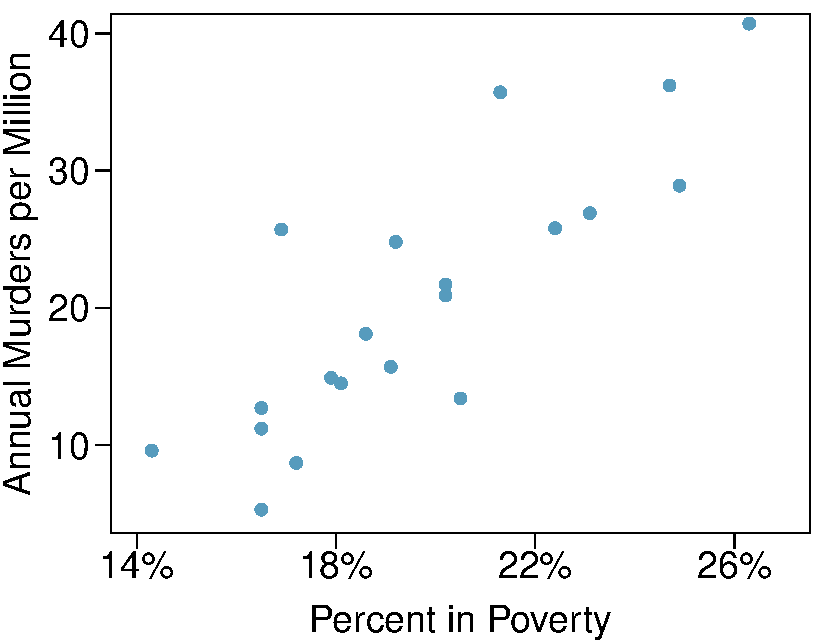
\includegraphics[width=\textwidth]{ch_regr_simple_linear/figures/eoce/murders_poverty_reg/murders_poverty.pdf}
\end{minipage}
}{}

% 26

\eoce{\qt{Cats, Part I\label{cat_body_heart_reg}} The following regression output is 
for predicting the heart weight (in g) of cats from their body weight 
(in kg). The coefficients are estimated using a dataset of 144 
domestic cats.\\[2mm]
\begin{minipage}[c]{0.56\textwidth}
{\footnotesize
\begin{tabular}{rrrrr}
    \hline
            & Estimate  & Std. Error    & t value   & Pr($>$$|$t$|$) \\ 
    \hline
(Intercept) & -0.357    & 0.692         & -0.515    & 0.607 \\ 
body wt     & 4.034     & 0.250         & 16.119    & 0.000 \\ 
    \hline
\end{tabular}
$s = 1.452 \hfill R^2 = 64.66\% \hfill R^2_{adj} = 64.41\%$ 
}
\begin{parts}
\item Write out the linear model.
\item Interpret the intercept.
\item Interpret the slope.
\item Interpret $R^2$.
\item Calculate the correlation coefficient.
\end{parts}
\end{minipage}
\begin{minipage}[c]{0.02\textwidth}
$\:$\\
\end{minipage}
\begin{minipage}[c]{0.39\textwidth}
\includegraphics[width=\textwidth]{ch_regr_simple_linear/figures/eoce/cat_body_heart_reg/cat_body_heart.pdf}
\end{minipage}
}{}
}








%__________________
\section{Types of outliers in linear regression}
\label{typesOfOutliersInLinearRegression}

In this section, we identify criteria for determining which
outliers are important and influential.
Outliers in regression are observations that fall far from
the cloud of points.
These points are especially important because they can have
a strong influence on the least squares line. 

\begin{examplewrap}
\begin{nexample}{There are six plots shown in
    Figure~\ref{outlierPlots} along with the least squares
    line and residual plots.
    For~each scatterplot and residual plot pair,
    identify the outliers and note how they influence
    the least squares line.
    Recall that an outlier is any point that doesn't appear
    to belong with the vast majority of the other points.}
  \label{outlierPlotsExample}%
  \begin{itemize}
  %\setlength{\itemsep}{0mm}
  \item[(1)]
      There is one outlier far from the other points,
      though it only appears to slightly influence the~line.
  \item[(2)]
      There is one outlier on the right, though it is quite
      close to the least squares line, which suggests it
      wasn't very influential.
  \item[(3)]
      There is one point far away from the cloud, and this
      outlier appears to pull the least squares line up on
      the right;
      examine how the line around the primary cloud doesn't
      appear to fit very~well.
  \item[(4)]
      There is a primary cloud and then a small secondary
      cloud of four outliers.
      The secondary cloud appears to be influencing the line
      somewhat strongly, making the least square line fit
      poorly almost everywhere.
      There might be an interesting explanation for the dual
      clouds, which is something that could be investigated.
  \item[(5)]
      There is no obvious trend in the main cloud of points
      and the outlier on the right appears to largely control
      the slope of the least squares line.
  \item[(6)]
      There is one outlier far from the cloud.
      However, it falls quite close to the least squares line
      and does not appear to be very influential.
  \end{itemize}
\end{nexample}
\end{examplewrap}

\begin{figure}
  \centering
  \Figure{}{outlierPlots}
  \caption{Six plots, each with a least squares line and
      residual plot. All data sets have at least one outlier.}
\label{outlierPlots}
\end{figure}

Examine the residual plots in Figure~\ref{outlierPlots}.
You will probably find that there is some trend in the main
clouds of~(3) and~(4).
In these cases, the outliers influenced the slope of the
least squares lines.
In~(5), data with no clear trend were assigned a line with
a large trend simply due to one outlier (!).
 
\begin{onebox}{Leverage}
  Points that fall horizontally away from the center of the
  cloud tend to pull harder on the line, so we call them points
  with \term{high leverage}.\index{leverage}
\end{onebox}

Points that fall horizontally far from the line are points
of high leverage;
these points can strongly influence the slope of the least
squares line.
If one of these high leverage points does appear to actually
invoke its influence on the slope of the line --
as in cases~(3), (4), and (5) of Example~\ref{outlierPlotsExample}
-- then we call it an \term{influential point}.
Usually we can say a point is influential if, had we fitted
the line without it, the influential point would have been
unusually far from the least squares line.

It is tempting to remove outliers.
Don't do this without a very good reason.
Models that ignore exceptional (and interesting) cases often
perform poorly.
For instance, if a financial firm ignored the largest market
swings -- the ``outliers'' --  they would soon go bankrupt
by making poorly thought-out investments.


{\exercisesheader{}

% 1

\eoce{\qt{Outliers, Part I\label{outliers_1}} Identify the outliers in the 
scatterplots shown below, and determine what type of outliers they are. 
Explain your reasoning.
\begin{center}
\includegraphics[width=0.32\textwidth]{ch_regr_simple_linear/figures/eoce/outliers_1/outliers_1_influential.pdf}
\includegraphics[width=0.32\textwidth]{ch_regr_simple_linear/figures/eoce/outliers_1/outliers_2_leverage.pdf}
\includegraphics[width=0.32\textwidth]{ch_regr_simple_linear/figures/eoce/outliers_1/outliers_3_outlier.pdf}
\end{center}
}{}

% 2

\eoce{\qt{Outliers, Part II\label{outliers_2}} Identify the outliers in the scatterplots 
shown below and determine what type of outliers they are. Explain 
your reasoning.
\begin{center}
\includegraphics[width=0.32\textwidth]{ch_regr_simple_linear/figures/eoce/outliers_2/outliers_1_influential.pdf}
\includegraphics[width=0.32\textwidth]{ch_regr_simple_linear/figures/eoce/outliers_2/outliers_2_influential.pdf}
\includegraphics[width=0.32\textwidth]{ch_regr_simple_linear/figures/eoce/outliers_2/outliers_3_outlier.pdf}
\end{center}
}{}

% 3

\eoce{\qt{Urban homeowners, Part I\label{urban_homeowners_outlier}} The 
scatterplot below shows the percent of families who own their 
home vs. the percent of the population living in urban areas.
\footfullcite{data:urbanOwner} There are 52 observations, each 
corresponding to a state in the US. Puerto Rico and District of 
Columbia are also included.

\noindent\begin{minipage}[c]{0.5\textwidth}
\begin{parts}
\item Describe the relationship between the percent of families who 
own their home and the percent of the population living in urban areas.
\item The outlier at the bottom right corner is District of Columbia, 
where 100\% of the population is considered urban. What type of an outlier 
is this observation?
\end{parts}
\end{minipage}
\begin{minipage}[c]{0.05\textwidth}
$\:$\\
\end{minipage}
\begin{minipage}[c]{0.4\textwidth}
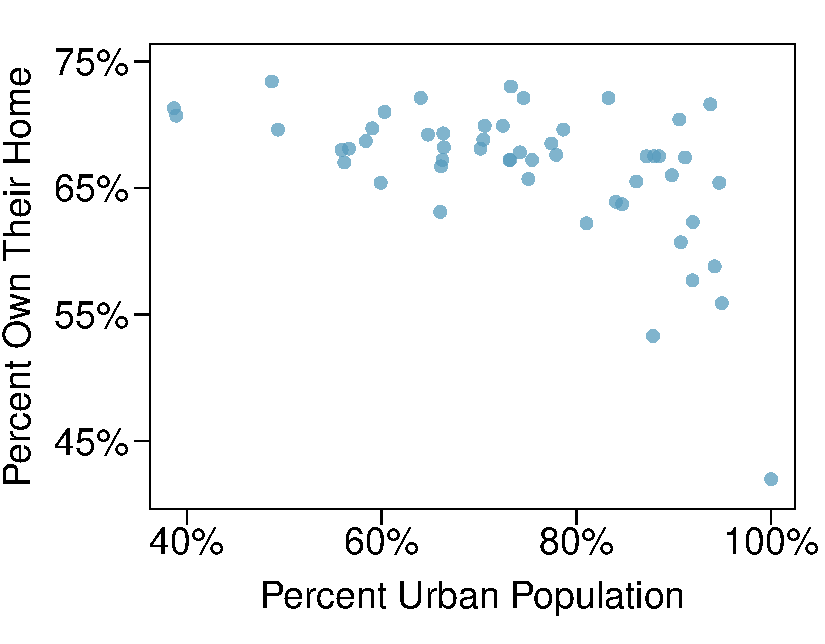
\includegraphics[width=0.95\textwidth]{ch_regr_simple_linear/figures/eoce/urban_homeowners_outlier/urban_homeowners_outlier.pdf} \vspace{-3mm}
\end{minipage}
}{}

% 4

\eoce{\qt{Crawling babies, Part II\label{crawling_babies_outlier}} 
Exercise~\ref{crawling_babies_corr_units} introduces 
data on the average monthly temperature during the month babies first 
try to crawl (about 6 months after birth) and the average first 
crawling age for babies born in a given month. A scatterplot of these 
two variables reveals a potential outlying month when the average 
temperature is about 53\degree F and average crawling age is about 
28.5 weeks. Does this point have high leverage? Is it an influential 
point?
}{}
}








%__________________
\section{Inference for linear regression}
\label{inferenceForLinearRegression}

In this section, we discuss uncertainty in the estimates
of the slope and y-intercept for a regression line.
Just as we identified standard errors for point estimates
in previous chapters, we first discuss standard errors for
these new estimates.


\subsection{Midterm elections and unemployment}

\index{data!midterm elections|(}

Elections for members of the United States House
of Representatives occur every two years, coinciding
every four years with the U.S. Presidential election.
The set of House elections occurring during the middle
of a Presidential term are called
\indexthis{midterm elections}{midterm election}.
In America's two-party system, one political theory
suggests the higher the unemployment rate, the worse
the President's party will do in the midterm elections.

To assess the validity of this claim, we can compile
historical data and look for a connection.
We consider every midterm election from 1898 to 2018,
with the exception of those elections during the Great
Depression.
Figure~\ref{unemploymentAndChangeInHouse} shows these data
and the least-squares regression line: \vspace{-2mm}
\begin{align*}
&\text{\% change in House seats for President's party}  \\
&\qquad\qquad= -7.36 - 0.89 \times \text{(unemployment rate)}
\end{align*}
We consider the percent change in the number of seats
of the President's party (e.g. percent change in the number
of seats for Republicans in 2018) against the unemployment
rate.

Examining the data, there are no clear deviations from
linearity, the constant variance condition,
or substantial outliers.
While the data are collected sequentially, a separate analysis
was used to check for any apparent correlation between successive
observations;
no such correlation was found.

\begin{figure}[h]
  \centering
  \Figure{}{unemploymentAndChangeInHouse}
  \caption{The percent change in House seats for the
      President's party in each election from 1898 to 2010
      plotted against the unemployment rate.
      The two points for the Great Depression have been
      removed, and a least squares regression line has been
      fit to the data.}
  \label{unemploymentAndChangeInHouse}
\end{figure}

\begin{exercisewrap}
\begin{nexercise}
The data for the Great Depression (1934 and 1938) were removed
because the unemployment rate was 21\% and 18\%, respectively.
Do you agree that they should be removed for this investigation?
Why or why not?\footnotemark{}
\end{nexercise}
\end{exercisewrap}
\footnotetext{We will provide two considerations.
  Each of these points would have very high leverage on any
  least-squares regression line, and years with such high
  unemployment may not help us understand what would happen
  in other years where the unemployment is only modestly high.
  On the other hand, these are exceptional cases, and we would
  be discarding important information if we exclude them from
  a final analysis.}

There is a negative slope in the line shown in
Figure~\ref{unemploymentAndChangeInHouse}.
However, this slope (and the y-intercept) are only estimates
of the parameter values.
We might wonder, is this convincing evidence that the ``true''
linear model has a negative slope?
That is, do the data provide strong evidence that the political
theory is accurate, where the unemployment rate is a useful
predictor of the midterm election?
We can frame this investigation into a statistical hypothesis
test:
\begin{itemize}
\item[$H_0$:]
    $\beta_1 = 0$.
    The true linear model has slope zero.
\item[$H_A$:]
    $\beta_1 \neq 0$.
    The true linear model has a slope different than zero.
    The unemployment is predictive of whether the President's
    party wins or loses seats in the House of Representatives.
\end{itemize}
We would reject $H_0$ in favor of $H_A$ if the data provide
strong evidence that the true slope parameter is different
than zero.
To assess the hypotheses, we identify a standard error
for the estimate, compute an appropriate test statistic,
and identify the p-value.


\subsection{Understanding regression output from software}
\label{testStatisticForTheSlope}

\newcommand{\midtermshouseDF}{27}

Just like other point estimates we have seen before,
we can compute a standard error and test statistic for $b_1$.
We will generally label the test statistic using a $T$,
since it follows the $t$-distribution.

We will rely on statistical software to compute the standard
error and leave the explanation of how this standard error
is determined to a second or third statistics course.
Figure~\ref{midtermUnempRegTable} shows software output for
the least squares regression line in
Figure~\ref{unemploymentAndChangeInHouse}.
The row labeled \emph{unemp} includes the point estimate
and other hypothesis test information for the slope,
which is the coefficient of the unemployment variable.

\begin{figure}[ht]
\centering
\begin{tabular}{rrrrr}
  \hline
  \vspace{-3.7mm} & & & & \\
  & Estimate & Std. Error & t value & Pr($>$$|$t$|$) \\ 
  \hline
  \vspace{-3.6mm} & & & & \\
  (Intercept) & -7.3644 & 5.1553 & -1.43 & 0.1646 \\ 
  unemp & -0.8897 & 0.8350 & -1.07 & 0.2961 \\ 
  \hline
  \multicolumn{5}{r}{$df=\midtermshouseDF{}$} \\
\end{tabular}
\caption{Output from statistical software for the regression
    line modeling the midterm election losses for the
    President's party as a response to unemployment.}
\label{midtermUnempRegTable}
\end{figure}

\begin{examplewrap}
\begin{nexample}{What do the first and second columns
    of Figure~\ref{midtermUnempRegTable} represent?}
  The entries in the first column represent the least
  squares estimates, $b_0$ and $b_1$, and the values in
  the second column correspond to the standard errors
  of each estimate.
  Using the estimates, we could write the equation
  for the least square regression line as
  \begin{align*}
  \hat{y} = -7.3644 - 0.8897 x
  \end{align*}
  where $\hat{y}$ in this case represents the predicted
  change in the number of seats for the president's party,
  and $x$ represents the unemployment rate.
\end{nexample}
\end{examplewrap}

\D{\newpage}

We previously used a $t$-test statistic for hypothesis testing
in the context of numerical data.
Regression is very similar.
In the hypotheses we consider, the null value for the slope is~0,
so we can compute the test statistic using the T (or Z) score
formula:
\begin{align*}
T
  = \frac{\text{estimate} - \text{null value}}{\text{SE}}
  = \frac{-0.8897 - 0}{0.8350}
  = -1.07
\end{align*}
This corresponds to the third column of
Figure~\ref{midtermUnempRegTable}.

%\begin{figure}[h]
%  \centering
%  \Figure{0.82}{pValueMidtermUnemp}
%  \caption{The distribution shown here is the sampling distribution for $b_1$, if the null hypothesis was true. The shaded tail represents the p-value for the hypothesis test evaluating whether there is convincing evidence that higher unemployment corresponds to a greater loss of House seats for the President's party during a midterm election.}
%  \label{pValueMidtermUnemp}
%\end{figure}

\begin{examplewrap}
\begin{nexample}{Use the table in
    Figure~\ref{midtermUnempRegTable}
    to determine the p-value for the hypothesis test.}
  The last column of the table gives the p-value for
  the two-sided hypothesis test for the coefficient of
  the unemployment rate: 0.2961.
  That is, the data do not provide convincing evidence
  that a higher unemployment rate has any correspondence
  with smaller or larger losses for the President's party
  in the House of Representatives in midterm elections.
\end{nexample}
\end{examplewrap}

\index{data!midterm elections|)}

\begin{onebox}{Inference for regression}
  We usually rely on statistical software to identify point
  estimates, standard errors, test statistics, and p-values
  in practice.
  However, be aware that software will not generally
  check whether the method is appropriate, meaning we must
  still verify conditions are met.
\end{onebox}

\begin{examplewrap}
\begin{nexample}{Examine Figure~\vref{elmhurstScatterWLSROnly},
    which relates the Elmhurst College aid and student family
    income.
    How sure are you that the slope is statistically
    significantly different from zero?
    That is, do you think a formal hypothesis test would reject
    the claim that the true slope of the line should be zero?}
  \label{overallAidIncomeInfAssessOfRegrLineSlope}%
  While the relationship between the variables is not perfect,
  there is an evident decreasing trend in the data.
  This suggests the hypothesis test will reject the null claim
  that the slope is zero.
\end{nexample}
\end{examplewrap}

\begin{exercisewrap}
\begin{nexercise}
Figure~\ref{rOutputForIncomeAidLSRLineInInferenceSection}
shows statistical software output from fitting the least
squares regression line shown in
Figure~\ref{elmhurstScatterWLSROnly}.
Use this output to formally evaluate the following
hypotheses.\footnotemark{}
\begin{itemize}
\setlength{\itemsep}{0mm}
\item[$H_0$:]
    The true coefficient for family income is zero.
\item[$H_A$:]
    The true coefficient for family income is not zero.
\end{itemize}
\end{nexercise}
\end{exercisewrap}
\footnotetext{We look in the second row corresponding
  to the family income variable.
  We see the point estimate of the slope of the line is -0.0431,
  the standard error of this estimate is 0.0108, and the $t$-test
  statistic is $T = -3.98$.
  The p-value corresponds exactly to the two-sided test we are
  interested in: 0.0002.
  The p-value is so small that we reject the null hypothesis
  and conclude that family income and financial aid at Elmhurst
  College for freshman entering in the year 2011 are negatively
  correlated and the true slope parameter is indeed less than~0,
  just as we believed in
  Example~\ref{overallAidIncomeInfAssessOfRegrLineSlope}.}

\begin{figure}[ht]
\centering
\begin{tabular}{rrrrr}
  \hline
  \vspace{-3.7mm} & & & & \\
 & Estimate & Std. Error & t value & Pr($>$$|$t$|$) \\ 
  \hline
  \vspace{-3.6mm} & & & & \\
(Intercept) & 24319.3 & 1291.5 & 18.83 & $<$0.0001 \\ 
family\us{}income & -0.0431 & 0.0108 & -3.98 & 0.0002 \\ 
   \hline
   \multicolumn{5}{r}{$df=48$} \\
\end{tabular}
\caption{Summary of least squares fit for the Elmhurst
    College data, where we are predicting the gift aid
    by the university based on the family income of
    students.}
\label{rOutputForIncomeAidLSRLineInInferenceSection}
\end{figure}


\newpage

\subsection{Confidence interval for a coefficient}

\index{confidence interval!regression|(}%

Similar to how we can conduct a hypothesis test for
a model coefficient using regression output, we can also
construct a confidence interval for that coefficient.

\begin{examplewrap}
\begin{nexample}{
    Compute the 95\% confidence interval for the
    \var{family\us{}income} coefficient using the
    regression output from
    Table~\ref{rOutputForIncomeAidLSRLineInInferenceSection}.}
  The point estimate is -0.0431 and the standard error is
  $SE = 0.0108$.
  When constructing a confidence interval for a model
  coefficient, we generally use a $t$-distribution.
  The degrees of freedom for the distribution are noted in
  the regression output, $df = 48$, allowing us to identify
  $t_{48}^{\star} = 2.01$ for use in the confidence interval.

  We can now construct the confidence interval in the usual way:
  \begin{align*}
  \text{point estimate} \pm t_{48}^{\star} \times SE
    \qquad\to\qquad -0.0431 \pm 2.01 \times 0.0108
    \qquad\to\qquad (-0.0648, -0.0214)
  \end{align*}
  We are 95\% confident that with each dollar increase in
  \var{family\us{}income}, the university's gift aid is
  predicted to decrease on average by \$0.0214 to \$0.0648.
\end{nexample}
\end{examplewrap}

\begin{onebox}{Confidence intervals for coefficients}
  Confidence intervals for model coefficients can be computed
  using the $t$-distribution:
  \begin{align*}
  b_i \ \pm\ t_{df}^{\star} \times SE_{b_{i}}
  \end{align*}
  where $t_{df}^{\star}$ is the appropriate $t$-value
  corresponding to the confidence level with the
  model's degrees of freedom.
\end{onebox}

On the topic of intervals in this book, we've focused exclusively
on confidence intervals for model parameters.
However, there are other types of intervals that may be
of interest, including
prediction intervals\index{prediction interval}
for a response value
and also
confidence intervals for a
mean response value\index{mean response value}
in the context of regression.
These two interval types are introduced in an online extra
that you may download at
\begin{center}
\oiRedirect{stat_extra_linear_regression_supp}
    {www.openintro.org/d?file=stat\_extra\_linear\_regression\_supp}
\end{center}

\index{confidence interval!regression|)}%
\index{regression|)}


{


%_______________
\newpage\subsection*{Exercises} % Inference for linear regression

% 1

\eoce{\qt{Body measurements, Part IV\label{body_measurements_weight_height_inf}} 
The scatterplot and least squares summary below show the relationship 
between weight measured in kilograms and height measured in centimeters 
of 507 physically active individuals.

\noindent\begin{minipage}[c]{0.4\textwidth}
\begin{center}
\includegraphics[width=\textwidth]{ch_regr_simple_linear/figures/eoce/body_measurements_weight_height_inf/body_measurements_weight_height.pdf}
\end{center}
\end{minipage}
\begin{minipage}[c]{0.6\textwidth}
{\scriptsize
\begin{center}
\begin{tabular}{rrrrr}
    \hline
            & Estimate  & Std. Error    & t value   & Pr($>$$|$t$|$) \\ 
    \hline
(Intercept) & -105.0113 & 7.5394        & -13.93    & 0.0000 \\ 
height      & 1.0176    & 0.0440        & 23.13     & 0.0000 \\
    \hline
\end{tabular}
\end{center}
}
\end{minipage}
\begin{parts}
\item Describe the relationship between height and weight.
\item Write the equation of the regression line. Interpret the slope 
and intercept in context.
\item Do the data provide strong evidence that an increase in height 
is associated with an increase in weight? State the null and alternative 
hypotheses, report the p-value, and state your conclusion.
\item The correlation coefficient for height and weight is 0.72. 
Calculate $R^2$ and interpret it in context.
\end{parts}
}{}

% 2

\eoce{\qt{Beer and blood alcohol content\label{beer_blood_alcohol_inf}} 
Many people believe that gender, 
weight, drinking habits, and many other factors are much more important 
in predicting blood alcohol content (BAC) than simply considering the 
number of drinks a person consumed. Here we examine data from sixteen 
student volunteers at Ohio State University who each drank a randomly 
assigned number of cans of beer. These students were evenly divided 
between men and women, and they differed in weight and drinking habits. 
Thirty minutes later, a police officer measured their blood alcohol 
content (BAC) in grams of alcohol per deciliter of blood.
\footfullcite{Malkevitc+Lesser:2008} The scatterplot and regression 
table summarize the findings.

\noindent\begin{minipage}[c]{0.4\textwidth}
\begin{center}
\includegraphics[width=\textwidth]{ch_regr_simple_linear/figures/eoce/beer_blood_alcohol_inf/beer_blood_alcohol.pdf}
\end{center}
\end{minipage}
\begin{minipage}[c]{0.6\textwidth}
{\scriptsize
\begin{center}
\begin{tabular}{rrrrr}
    \hline
            & Estimate  & Std. Error    & t value   & Pr($>$$|$t$|$) \\ 
    \hline
(Intercept) & -0.0127   & 0.0126        & -1.00     & 0.3320 \\ 
beers       & 0.0180    & 0.0024        & 7.48      & 0.0000 \\ 
    \hline
\end{tabular}
\end{center}
}
\end{minipage}
\begin{parts}
\item Describe the relationship between the number of cans of beer 
and BAC.
\item Write the equation of the regression line. Interpret the slope 
and intercept in context.
\item Do the data provide strong evidence that drinking more cans of 
beer is associated with an increase in blood alcohol? State the null 
and alternative hypotheses, report the p-value, and state your 
conclusion.
\item The correlation coefficient for number of cans of beer and BAC 
is 0.89. Calculate $R^2$ and interpret it in context.
\item Suppose we visit a bar, ask people how many drinks they have had, 
and also take their BAC. Do you think the relationship between number 
of drinks and BAC would be as strong as the relationship found in the 
Ohio State study?
\end{parts}
}{}

% 3

\eoce{\qt{Husbands and wives, Part II\label{husbands_wives_height_inf}} The 
scatterplot below summarizes husbands' and wives' heights in a random 
sample of 170 married couples in Britain, where both partners' ages are 
below 65 years. Summary output of the least squares fit for predicting 
wife's height from husband's height is also provided in the table.

\noindent\begin{minipage}[c]{0.4\textwidth}
\begin{center}
\includegraphics[width=\textwidth]{ch_regr_simple_linear/figures/eoce/husbands_wives_height_inf/husbands_wives_height.pdf}
\end{center}
\end{minipage}
\begin{minipage}[c]{0.6\textwidth}
{\scriptsize
\begin{center}
\begin{tabular}{rrrrr}
    \hline
                    & Estimate  & Std. Error    & t value   & Pr($>$$|$t$|$) \\ 
    \hline
(Intercept)         & 43.5755   & 4.6842        & 9.30      & 0.0000 \\ 
height\_\hspace{0.3mm}husband   & 0.2863    & 0.0686        & 4.17      & 0.0000 \\ 
    \hline
\end{tabular}
\end{center}
}
\end{minipage}
\begin{parts}
\item Is there strong evidence that taller men marry taller women? 
State the hypotheses and include any information used to conduct the test.
\item Write the equation of the regression line for predicting wife's 
height from husband's height.
\item Interpret the slope and intercept in the context of the application.
\item Given that $R^2 = 0.09$, what is the correlation of heights 
in this data set?
\item You meet a married man from Britain who is 5'9" (69 inches). 
What would you predict his wife's height to be? How reliable is this 
prediction?
\item You meet another married man from Britain who is 6'7" (79 inches). 
Would it be wise to use the same linear model to predict his wife's 
height? Why or why not?
\end{parts}
}{}

% 4

\eoce{\qt{Husbands and wives, Part III\label{husbands_wives_age_inf}}
Exercise~\ref{husbands_wives_height_inf} presents a scatterplot displaying the 
relationship between husbands' and wives' ages in a random sample of 
170 married couples in Britain, where both partners' ages are below 65 
years. Given below is summary output of the least squares fit for 
predicting wife's age from husband's age.

\noindent\begin{minipage}[c]{0.4\textwidth}
\begin{center}
\includegraphics[width=\textwidth]{ch_regr_simple_linear/figures/eoce/husbands_wives_age_inf/husbands_wives_age.pdf}
\end{center}
\end{minipage}
\begin{minipage}[c]{0.6\textwidth}
{\scriptsize
\begin{center}
\begin{tabular}{rrrrr}
  \hline
                & Estimate  & Std. Error    & t value   & Pr($>$$|$t$|$) \\ 
  \hline
(Intercept)     & 1.5740    & 1.1501        & 1.37      & 0.1730 \\ 
age\_\hspace{0.3mm}husband  & 0.9112    & 0.0259        & 35.25     & 0.0000 \\ 
   \hline
\multicolumn{5}{r}{$df = 168$} \\
\end{tabular}
\end{center}
}
\end{minipage}
\begin{parts}
\item We might wonder, is the age difference between husbands and 
wives consistent across ages? If this were the case, then the slope 
parameter would be $\beta_1 = 1$. Use the information above to evaluate 
if there is strong evidence that the difference in husband and wife ages 
differs for different ages.
\item Write the equation of the regression line for predicting wife's 
age from husband's age.
\item Interpret the slope and intercept in context.
\item Given that $R^2 = 0.88$, what is the correlation of ages  in 
this data set?
\item You meet a married man from Britain who is 55 years old. What 
would you predict his wife's age to be? How reliable is this prediction?
\item You meet another married man from Britain who is 85 years old. 
Would it be wise to use the same linear model to predict his wife's 
age? Explain.
\end{parts}
}{}

% 5

\eoce{$\:$ \\
\noindent \begin{minipage}[c]{0.56\textwidth}
\qt{Urban homeowners, Part II\label{urban_homeowners_cond}}
\textbf{\color{red}FINAL FORMATTING REQUIRED.}
Exercise~\ref{urban_homeowners_outlier} gives a scatterplot displaying the 
relationship between the percent of families that own their home and 
the percent of the population living in urban areas. Below is a 
similar scatterplot, excluding District of Columbia, as well as the 
residuals plot. There were 51 cases.
\begin{parts}
\item For these data, $R^2=0.28$. What is the correlation? How can 
you tell if it is positive or negative?
\item Examine the residual plot. What do you observe? Is a simple 
least squares fit appropriate for these data?
\end{parts}
\vspace{15mm}
\end{minipage}
\begin{minipage}[c]{0.02\textwidth}
$\:$ \\
\end{minipage}
\begin{minipage}[c]{0.4\textwidth}
\begin{center}
\includegraphics[width=\textwidth]{ch_regr_simple_linear/figures/eoce/urban_homeowners_cond/urban_homeowners_cond.pdf}
\end{center}
\end{minipage}
}{}

% 6

\eoce{\qt{Rate my professor\label{rate_my_prof}} Many college courses conclude by giving 
students the opportunity to evaluate the course and the instructor 
anonymously. However, the use of these student evaluations as an 
indicator of course quality and teaching effectiveness is often 
criticized because these measures may reflect the influence of non-
teaching related characteristics, such as the physical appearance of 
the instructor. Researchers at University of Texas, Austin collected 
data on teaching evaluation score (higher score means better) and 
standardized beauty score (a score of 0 means average, negative score 
means below average, and a positive score means above average) for a 
sample of 463 professors.\footfullcite{Hamermesh:2005} The 
scatterplot below shows the relationship between these variables, and 
also provided is a regression output for predicting teaching 
evaluation score from beauty score.

\noindent\begin{minipage}[c]{0.4\textwidth}
\includegraphics[width=\textwidth]{ch_regr_simple_linear/figures/eoce/rate_my_prof/rate_my_prof_eval_beauty.pdf} \\
\end{minipage}
\begin{minipage}[c]{0.6\textwidth}
\begin{tabular}{rrrrr}
    \hline
            & Estimate  & Std. Error    & t value   & Pr($>$$|$t$|$) \\ 
  \hline
(Intercept) & 4.010     & 0.0255        & 	157.21  & 0.0000 \\ 
beauty      &  \fbox{\textcolor{white}{{\footnotesize Cell 1}}}  
                        & 0.0322        & 4.13      & 0.0000\vspace{0.8mm} \\ 
   \hline
\end{tabular}
\end{minipage}
\begin{parts}
\item Given that the average standardized beauty score is -0.0883 and 
average teaching evaluation score is 3.9983, calculate the slope. 
Alternatively, the slope may be computed using just the information 
provided in the model summary table.
\item Do these data provide convincing evidence that the slope of the 
relationship between teaching evaluation and beauty is positive? 
Explain your reasoning.
\item List the conditions required for linear regression and check if 
each one is satisfied for this model based on the following 
diagnostic plots.
\begin{center}
\includegraphics[width=0.4\textwidth]{ch_regr_simple_linear/figures/eoce/rate_my_prof/rate_my_prof_residuals.pdf}
\includegraphics[width=0.4\textwidth]{ch_regr_simple_linear/figures/eoce/rate_my_prof/rate_my_prof_residuals_hist.pdf} \\
\includegraphics[width=0.4\textwidth]{ch_regr_simple_linear/figures/eoce/rate_my_prof/rate_my_prof_residuals_qq.pdf}
\includegraphics[width=0.4\textwidth]{ch_regr_simple_linear/figures/eoce/rate_my_prof/rate_my_prof_residuals_order.pdf}
\end{center}
\end{parts}
}{}

% 7

\eoce{\qt{Murders and poverty, Part II\label{murders_poverty_inf}}
Exercise~\ref{murders_poverty_reg} presents regression output from a model 
for predicting annual murders per million from percentage living in 
poverty based on a random sample of 20 metropolitan areas. The model 
output is also provided below.
\begin{center}
\begin{tabular}{rrrrr}
    \hline
            & Estimate  & Std. Error    & t value   & Pr($>$$|$t$|$) \\ 
    \hline
(Intercept) & -29.901   & 7.789         & -3.839    & 0.001 \\ 
poverty\%   & 2.559     & 0.390         & 6.562     & 0.000 \\ 
    \hline
\end{tabular}
\[ s = 5.512 \qquad R^2 = 70.52\% \qquad R^2_{adj} = 68.89\% \]
\end{center}
\begin{parts}
\item What are the hypotheses for evaluating whether poverty percentage 
is a significant predictor of murder rate?
\item State the conclusion of the hypothesis test from part (a) in 
context of the data.
\item Calculate a 95\% confidence interval for the slope of poverty 
percentage, and interpret it in context of the data.
\item Do your results from the hypothesis test and the confidence 
interval agree? Explain.
\end{parts}
}{}

% 8

\eoce{\qt{Babies\label{babies_head_gestation_inf}} Is the gestational age 
(time between conception and birth) of a low birth-weight baby useful 
in predicting head circumference at birth? Twenty-five low birth-weight 
babies were studied at a Harvard teaching hospital; the investigators 
calculated the regression of head circumference (measured in centimeters) 
against gestational age (measured in weeks). The estimated regression 
line is
\[ \widehat{head~circumference} = 3.91 + 0.78 \times gestational~age \]
\begin{parts}
\item What is the predicted head circumference for a baby whose 
gestational age is 28 weeks?
\item The standard error for the coefficient of gestational age is 0.
35, which is associated with $df=23$. Does the model provide strong 
evidence that gestational age is significantly associated with head 
circumference?
\end{parts} 
}{}
}
